% XFed-IDS-ByzAgent -- IEEE conference paper (body) + complete-record appendices.
% Build: tectonic main.tex                 -> main.pdf (body + appendices)
%        tectonic main_conference.tex      -> main_conference.pdf (body + references only)
% Every number carries a trailing src comment naming the repo file it was copied from.
% paper/number_check.py re-checks each one against that file and writes number_check.md.
\documentclass[conference]{IEEEtran}
\IEEEoverridecommandlockouts
\usepackage[T1]{fontenc}
\usepackage{amsmath}
\usepackage{newtxtext,newtxmath}
\usepackage{cite}
\usepackage{graphicx}
\usepackage{booktabs}
\usepackage{array}
\usepackage{tabularx}
\usepackage{multirow}
\usepackage{xcolor}
% Okabe-Ito palette (colour-blind safe); used only for figure fills, never for text or links.
\definecolor{oiblue}{HTML}{0072B2}
\definecolor{oiorange}{HTML}{E69F00}
\definecolor{oigreen}{HTML}{009E73}
\definecolor{oivermillion}{HTML}{D55E00}
\definecolor{oisky}{HTML}{56B4E9}
\usepackage{tikz}
\usetikzlibrary{arrows.meta,positioning,fit,calc}
\usepackage[hidelinks]{hyperref}
\usepackage{url}
\def\UrlBreaks{\do\/\do-\do_\do.}

% ---- full version (body + appendices) unless main_conference.tex defines \conferenceonly
\newif\iffullversion
\ifdefined\conferenceonly \fullversionfalse \else \fullversiontrue \fi
\newcommand{\fullref}[1]{\iffullversion Appendix~\ref{#1}\else the extended version\fi}
% (no data numbers above this line)
\newcommand{\cmark}{\checkmark}
\newcommand{\pp}{\,pp}

\begin{document}

% Line break between author rows in IEEEtran's conference author layout.
\makeatletter
\newcommand{\linebreakand}{%
  \end{@IEEEauthorhalign}
  \hfill\mbox{}\par
  \mbox{}\hfill\begin{@IEEEauthorhalign}}
\makeatother

\title{Do Federated Intrusion Detectors Agree on Why?\\[4pt]
{\Large\normalfont Explanation Agreement and Client Trust under Non-IID Data on Corrected CICIDS2017}}

\author{%
\IEEEauthorblockN{V Naga Adithya}
\IEEEauthorblockA{Reg. No. 23BCE9062\\
\textit{School of Computer Science}\\
\textit{and Engineering, VIT-AP University}\\
Amaravati, India\\
{\footnotesize\texttt{adithya.23bce9062@vitapstudent.ac.in}}}
\and
\IEEEauthorblockN{T Shaun}
\IEEEauthorblockA{Reg. No. 23BCE9916\\
\textit{School of Computer Science}\\
\textit{and Engineering, VIT-AP University}\\
Amaravati, India\\
{\footnotesize\texttt{shaun.23bce9916@vitapstudent.ac.in}}}
\and
\IEEEauthorblockN{P Sampath}
\IEEEauthorblockA{Reg. No. 23BCE8614\\
\textit{School of Computer Science}\\
\textit{and Engineering, VIT-AP University}\\
Amaravati, India\\
{\footnotesize\texttt{sampath.23bce8614@vitapstudent.ac.in}}}
\linebreakand
\IEEEauthorblockN{D Tharun}
\IEEEauthorblockA{Reg. No. 23BCE8818\\
\textit{School of Computer Science}\\
\textit{and Engineering, VIT-AP University}\\
Amaravati, India\\
{\footnotesize\texttt{tharun.23bce8818@vitapstudent.ac.in}}}
\and
\IEEEauthorblockN{Prof. Gargi Madala (Guide)}
\IEEEauthorblockA{\textit{School of Computer Science}\\
\textit{and Engineering, VIT-AP University}\\
Amaravati, India}
}

\maketitle

% =====================================================================================
\begin{abstract}
Federated learning lets organisations train one network intrusion detector without
pooling their traffic. Two questions are usually left open: do the participants'
models flag attacks for the same reasons, and is any participant poisoning the shared
model? We examine both in one system built on the corrected CICIDS2017 data (Distrinet
V4), spread over ten silos with Dirichlet label skew $\alpha\in\{0.1,0.5,5.0\}$ and three % src: PROJECT_INSTRUCTIONS.md; docs/contribution_a_results.md; docs/contribution_b_results.md; data/README.md; docs/preregistration_accuracy.md; docs/efficiency_results.md
seeds. FedAvg reaches test macro-F1 of 0.516\,$\pm$\,0.048, 0.941\,$\pm$\,0.057 and % src: PROJECT_INSTRUCTIONS.md
0.990\,$\pm$\,0.001. Client-side SHAP rankings match the global model at median % src: PROJECT_INSTRUCTIONS.md
Jaccard@10 of 0.333, 0.538 and 0.667, against a chance level of 0.065 and a % src: PROJECT_INSTRUCTIONS.md
seed-noise floor of 0.429 measured between centralized models that differ only by % src: PROJECT_INSTRUCTIONS.md
seed. The $\alpha=0.1$ value lies under that floor, but the result is directional, not % src: PROJECT_INSTRUCTIONS.md; docs/contribution_a_results.md; docs/contribution_b_results.md; data/README.md; docs/preregistration_accuracy.md; docs/efficiency_results.md
significant: its cluster-bootstrap interval [0.250, 0.429] touches the floor range. % src: PROJECT_INSTRUCTIONS.md
In a separate experiment, a language-model trust agent (ByzAgent) reads per-silo
training statistics under a worst-case label-flipping attack. It produces decisions
plus a rationale of measured fidelity, and part of what it flags is silo composition
rather than attack. Multi-Krum excluded a malicious silo 0\% of the time. % src: PROJECT_INSTRUCTIONS.md
\end{abstract}

\begin{IEEEkeywords}
Federated learning, intrusion detection, explainable artificial intelligence,
Byzantine robustness, large language models
\end{IEEEkeywords}
\begingroup\renewcommand{\thefootnote}{}
\footnotetext{B.Tech CSE and Specializations, Capstone Project, Fall 2026-27. % numcheck: ignore
Registration numbers: V Naga Adithya 23BCE9062, T Shaun 23BCE9916, % numcheck: ignore
P Sampath 23BCE8614, D Tharun 23BCE8818.} % numcheck: ignore
\endgroup

% =====================================================================================
\section{Introduction}

A network intrusion detection system (IDS) learns what attacks look like from labelled
traffic, and no single organisation sees every kind of attack. Pooling flow records
across organisations would help the detector, but those records describe internal
hosts, users and services, so legal and contractual limits often rule it out.
Federated learning (FL) offers a way around this: each organisation trains on its own
traffic and only model weights travel to an aggregating server~\cite{mcmahan2017}.
Several groups have built FL-based detectors for IoT and enterprise
traffic~\cite{nguyen2019diot,rahman2020,mothukuri2022,campos2022,agrawal2022} and report
accuracy close to a centrally trained model.

Accuracy is usually where such evaluations stop. We think two further questions matter
to anyone who would run a federated IDS. The first is about explanations. An analyst who
receives an alert also wants to know which flow features drove it, and in a federation
each silo holds its own copy of the model, trained on its own skewed slice of traffic.
If those copies rely on different features, the explanation an analyst sees depends on
whose model was asked. Oki et al.~\cite{oki2024} showed that FL pulls per-site
explanations closer to those of a centrally trained detector. We ask how far that holds
as label skew grows, and how much disagreement one should expect from random seeds
alone. The second question is about the participants. The server only sees weight
updates, so a silo that relabels its own data can bend the shared
model~\cite{tolpegin2020,nguyen2020poison}. Byzantine-robust aggregation rules exist for
this case~\cite{blanchard2017,yin2018}, but they were designed around geometric
outliers, and a silo whose traffic is simply unusual can look like an outlier too.

We built one system with five stages (data, federated training, an explanation check, a
trust check and a dashboard) and report the two checks as separate experiments with
separate evidence. Our contributions are:
\begin{enumerate}
\item A measurement of silo-versus-global explanation agreement (Jaccard@10 and weighted
Kendall's $\tau$) across three levels of label skew for a FedAvg detector on corrected
CICIDS2017, read against two reference lines: the chance level and a
\emph{centralized-seed instability floor}, i.e., the agreement between centralized models
trained identically apart from their random seed
(Sections~\ref{sec:m-expl} and~\ref{sec:r-expl}).
\item An observational analysis that separates label skew from silo size, which the
Dirichlet partitioner ties together: KL divergence from the global label mix still
predicts agreement after conditioning on log size. We report that entropy was tried
first and failed this test (Section~\ref{sec:r-expl}).
\item A trust check that sets a language-model agent (ByzAgent) against three classical
aggregators, namely trimmed mean, Krum and Multi-Krum, under a worst-case label-flipping
attack.
All four mechanisms respond to silo composition. The classical rules did not single out
the attackers (Multi-Krum excluded a malicious silo 0\% of the time); ByzAgent's flags % src: PROJECT_INSTRUCTIONS.md
also responded to the attack where silos were not already saturated. We also audit how
often the agent's stated reasons match the numbers it was shown
(Sections~\ref{sec:m-trust} and~\ref{sec:r-trust}).
\item An evaluation protocol that selects every model and round on validation data, a
written audit of every way the test set was read, one preregistered optimizer
comparison, and serving and communication measurements for the deployed model
(Sections~\ref{sec:setup}, \ref{sec:r-acc} and~\ref{sec:r-eff}).
\end{enumerate}
We do not claim the combination of FL, intrusion detection and explainability as new;
recent work already combines
them~\cite{dong2022fedforest,thi2023xfedhunter,bilal2025,gholamrezazadeh2026}.

% =====================================================================================
\section{Related Work}

\subsection{Federated learning for intrusion detection}
FedAvg~\cite{mcmahan2017} remains the default aggregator, and most FL-IDS studies keep
it. D\"IoT~\cite{nguyen2019diot} trained device-type anomaly models across home
gateways; Rahman et al.~\cite{rahman2020} compared centralized, on-device and federated
training for IoT detection; Mothukuri et al.~\cite{mothukuri2022} and Popoola et
al.~\cite{popoola2022} used recurrent and deep models for IoT attacks and zero-day
botnets. Two reviews~\cite{campos2022,agrawal2022} collect the challenges that still
stand between FL-based detection and deployment. Benchmarks build non-IID splits with a
tunable degree of skew~\cite{hsu2019,li2022noniid}, and server-side remedies include proximal local
terms~\cite{li2020fedprox}, server momentum~\cite{hsu2019} and adaptive server
optimizers~\cite{reddi2021}. What these studies share is a single yardstick, detection
accuracy. None of them asks whether the silo models detect the same attack for the same
reason.

\subsection{Explainable IDS and federated XAI}
SHAP~\cite{lundberg2017} is the usual tool for attributing an IDS decision to flow
features~\cite{wang2020xai}. Surveys map the open problems of explainable
IDS~\cite{neupane2022}, and one of them argues for combining XAI with FL in IoT
detection~\cite{arisdakessian2023}. Warnecke et al.~\cite{warnecke2020} proposed
criteria, robustness among them, for judging explanation methods in security tasks. Federated systems that add explanations to an IDS have
appeared: FEDFOREST uses gradient-boosted trees~\cite{dong2022fedforest},
XFedHunter explains APT detection in SDN~\cite{thi2023xfedhunter}, and recent work
pairs FedAvg with SHAP or LIME on IoT traffic~\cite{bilal2025,gholamrezazadeh2026}.
These systems produce explanations, but they do not compare explanations across
participants. Oki et al.~\cite{oki2024} come closest: they measured the distance between
per-class feature sets of a distributed and a non-distributed IDS and found that FL
shrinks it. The FedXAI survey of Gholizade et al.~\cite{gholizade2026} lists the
behaviour of explanations on non-IID clients among the field's unsolved problems and
observes that there is still no agreed way to score how stable federated explanations
are.

\subsection{Stability and consistency of explanations}
Outside FL, attributions are known to move under small perturbations of the
input~\cite{ghorbani2019,alvarezmelis2018}, and sampling-based explainers carry their own
estimation noise~\cite{slack2021}. Watson et al.~\cite{watson2022} retrained identical
architectures with different seeds and data order and found low explanation consistency,
which means two models can disagree about reasons even when nothing about their data
differs. Krishna et al.~\cite{krishna2024} gave a quantitative definition of disagreement between
explanation methods and found that it is common in practice. For comparing full
rankings, a weighted form of Kendall's $\tau$~\cite{kendall1938,vigna2015} counts
discordant pairs near the top of the ranking more heavily than those near the bottom. Faithfulness is commonly checked by deleting or inserting the
highest-ranked inputs and tracking the model's score~\cite{petsiuk2018}. The gap we see
is that federated studies report agreement numbers without the seed-noise reference
that Watson et al.'s result implies they need.

\subsection{Byzantine-robust aggregation}
Krum and Multi-Krum~\cite{blanchard2017} pick the updates closest to their neighbours,
and coordinate-wise trimmed mean~\cite{yin2018} discards extreme values per parameter.
Bulyan~\cite{mhamdi2018} combines the two ideas. Later defences use a server-held root
dataset (FLTrust~\cite{cao2021fltrust}), the diversity of client updates over training
(FoolsGold~\cite{fung2020}), or iterative clipping with worker momentum that carries
information across rounds~\cite{karimireddy2021}.
Attack papers show that distance-based rules can be bypassed by crafted
updates~\cite{fang2020local}, and label flipping~\cite{tolpegin2020} and backdoor
injection have been shown for FL-based IoT detectors specifically~\cite{nguyen2020poison}.
Most evaluations assume that honest clients look alike. Under strong label skew they do
not, and the effect of this on what these rules exclude is rarely measured.

\subsection{Language-model agents for security decisions}
Agents that interleave reasoning with actions~\cite{yao2023react} have been applied to
penetration testing~\cite{deng2024pentestgpt} and to exploiting known
vulnerabilities~\cite{fang2024oneday}, and a recent review~\cite{xu2026llmsec} maps many
other security uses. A known weakness is that the reasons a model writes down need not
reflect what drove its answer~\cite{turpin2023}. If an agent is placed in an aggregation
loop, its written rationale therefore has to be checked against the data it was given,
not taken at face value.

\subsection{CICIDS2017 and its corrections}
CICIDS2017~\cite{sharafaldin2018} is widely used, but Engelen et al.~\cite{engelen2021}
documented errors in its flow construction, feature extraction and labelling, and Liu et
al.~\cite{liu2022} traced further errors through the dataset lifecycle and released the
refined version we use. Lanvin et al.~\cite{lanvin2023} corrected a separate set of
issues; we did not use that branch. Arp et al.~\cite{arp2022} list data snooping among
common pitfalls in security ML, which is why we audit our own test-set use.

\subsection{Positioning}
Our explanation check builds directly on Oki et al.~\cite{oki2024}. Where they found that
FL brings per-site explanations closer together, we vary label skew and look for the
point at which that effect gives out. We also measure something the FL-IDS papers above
leave out: the spread in feature rankings among centralized models whose only difference
is the seed. That spread is the yardstick a federated gap has to beat before it can be
blamed on federation, and it is one concrete answer to the missing consistency metrics
that Gholizade et al.~\cite{gholizade2026} point to. For the trust check, we run the
Krum family on a 10-silo federation with the true attacker count handed to it, and we % src: PROJECT_INSTRUCTIONS.md
score the agent's written reasons against the statistics it saw. The text summaries the
dashboard generates for analysts are a convenience, and we make no research claim about
them. Table~\ref{tab:related} sets out the comparison.

\begin{table}[t]
\centering
\caption{Closest works. A mark means the paper's abstract or text, as we read it, shows
the property: FL, IDS, explanations (XAI), an explanation-consistency metric (Cons.), a
seed-noise control (Seed), a Byzantine defence evaluated (Byz.), an LLM agent (LLM).}
\label{tab:related}
\footnotesize
\setlength{\tabcolsep}{2.6pt}
\begin{tabular}{@{}lccccccc@{}}
\toprule
Work & FL & IDS & XAI & Cons. & Seed & Byz. & LLM\\
\midrule
D\"IoT~\cite{nguyen2019diot} & \cmark & \cmark & & & & & \\
Nguyen et al.~\cite{nguyen2020poison} & \cmark & \cmark & & & & \cmark & \\
FLTrust~\cite{cao2021fltrust} & \cmark & & & & & \cmark & \\
FEDFOREST~\cite{dong2022fedforest} & \cmark & \cmark & \cmark & & & & \\
XFedHunter~\cite{thi2023xfedhunter} & \cmark & \cmark & \cmark & & & & \\
Oki et al.~\cite{oki2024} & \cmark & \cmark & \cmark & \cmark & & & \\
Bilal et al.~\cite{bilal2025} & \cmark & \cmark & \cmark & & & & \\
XAI FL-IDS~\cite{gholamrezazadeh2026} & \cmark & \cmark & \cmark & & & & \\
Watson et al.~\cite{watson2022} & & & \cmark & \cmark & \cmark & & \\
PentestGPT~\cite{deng2024pentestgpt} & & & & & & & \cmark\\
\midrule
This work & \cmark & \cmark & \cmark & \cmark & \cmark & \cmark & \cmark\\
\bottomrule
\end{tabular}
\end{table}

% =====================================================================================
\section{System Overview}
\label{sec:system}

Fig.~\ref{fig:pipeline} shows the five stages. \emph{Data}: the corrected CICIDS2017
flows are cleaned into eight attack families plus Benign and split once into training,
validation and test sets. \emph{Federated training}: ten silos train a shared multilayer
perceptron with Flower~\cite{beutel2020flower}; every silo trains in every round, and
the round kept is the one with the best validation score. \emph{Explanation check}:
each silo computes SHAP attributions locally and sends only top-$k$ feature indices to
the server, which compares them with the global model's ranking. \emph{Trust check}: the
server logs five statistics per silo and round; ByzAgent or a classical robust rule
decides how much each update counts. \emph{Dashboard}: a FastAPI backend serves the
selected model, explanations and trust decisions to a React front end
\iffullversion (Fig.~\ref{fig:dashlive})\fi.

\begin{figure}[t]
\centering
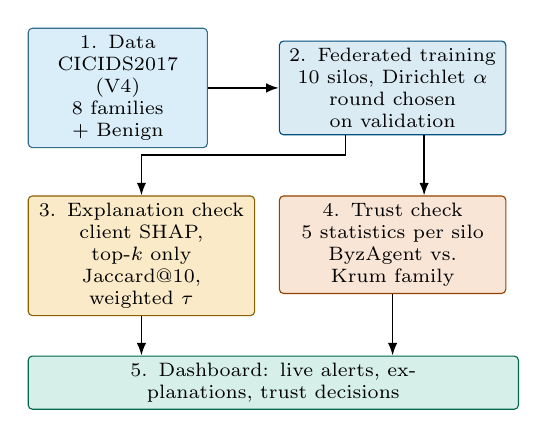
\begin{tikzpicture}[
  font=\scriptsize,
  box/.style={draw, rounded corners=1.5pt, align=center, inner sep=2.5pt, minimum height=9mm},
  arr/.style={-{Latex[length=1.6mm]}, semithick}]
\node[box, fill=oisky!22, draw=oisky!60!black, text width=21mm] (data) {1. Data\\CICIDS2017 (V4)\\8 families + Benign};
\node[box, fill=oiblue!14, draw=oiblue!70!black, text width=27mm, right=9mm of data] (fl) {2. Federated training\\10 silos, Dirichlet $\alpha$\\round chosen on validation};
\node[box, fill=oiorange!22, draw=oiorange!60!black, text width=27mm, below=6mm of data.south west, anchor=north west] (exp) {3. Explanation check\\client SHAP, top-$k$ only\\Jaccard@10, weighted $\tau$};
\node[box, fill=oivermillion!16, draw=oivermillion!70!black, text width=27mm, anchor=north east] (trust) at (fl.south east |- exp.north) {4. Trust check\\5 statistics per silo\\ByzAgent vs.\ Krum family};
\node[box, fill=oigreen!16, draw=oigreen!65!black, minimum height=6mm, anchor=north west, text width=60.5mm] (dash) at ($(exp.south west)+(0,-5mm)$) {5. Dashboard: live alerts, explanations, trust decisions};
\draw[arr] (data) -- (fl);
\draw[arr] (fl.south) ++(-6mm,0) -- ++(0,-2.5mm) -| (exp.north);
\draw[arr] (fl.south) ++(4mm,0) -- ($(trust.north)+(4mm,0)$);
\draw[arr] (exp.south) -- (exp.south |- dash.north);
\draw[arr] (trust.south) -- (trust.south |- dash.north);
\end{tikzpicture}
\caption{The five-stage pipeline. Stages 3 and 4 are separate experiments on the same % src: PROJECT_INSTRUCTIONS.md; docs/contribution_a_results.md; docs/contribution_b_results.md; data/README.md; docs/preregistration_accuracy.md; docs/efficiency_results.md
federated runs and are reported separately.}
\label{fig:pipeline}
\end{figure}

\iffullversion
\begin{figure}[t]
\centering
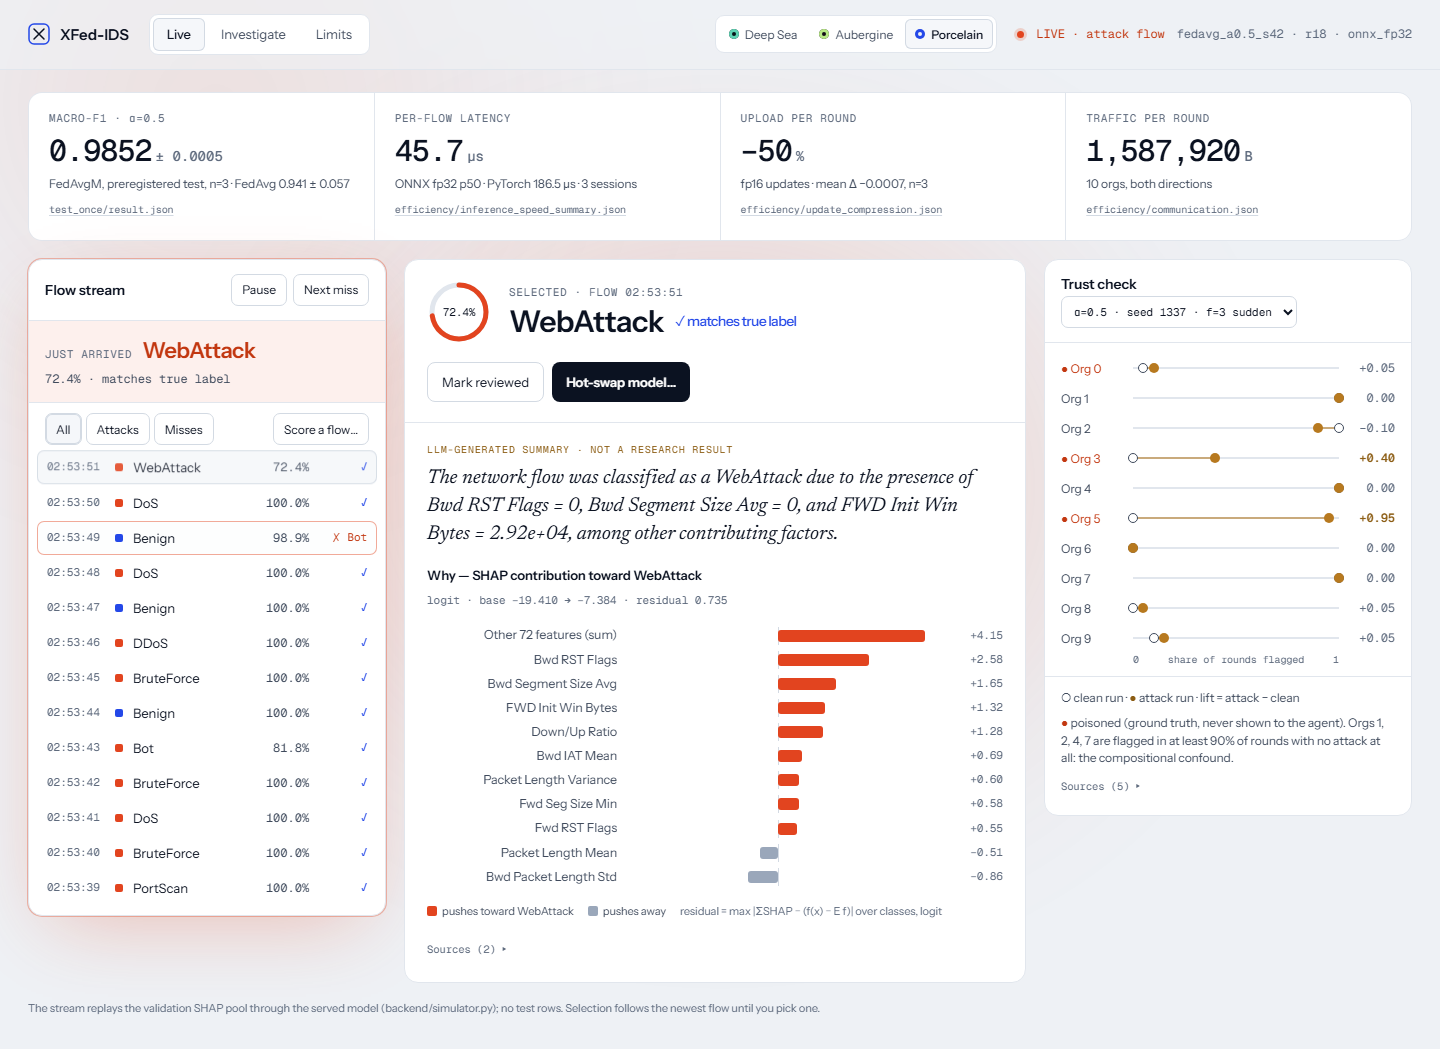
\includegraphics[width=\columnwidth]{figs/dash_live.png}
\caption{Dashboard, Live route: alert stream, one alert's SHAP contributions, and the trust panel.}
\label{fig:dashlive}
\end{figure}
\fi

% =====================================================================================
\section{Methodology}

\subsection{Data and partitioning}
We use the Distrinet CICIDS2017 release (version 4) of Liu et al.~\cite{liu2022}, % src: PROJECT_INSTRUCTIONS.md; docs/contribution_a_results.md; docs/contribution_b_results.md; data/README.md; docs/preregistration_accuracy.md; docs/efficiency_results.md
which builds on the corrections of Engelen et al.~\cite{engelen2021}. The raw files hold
2,099,976 flows with 82 numeric features once seven identifier columns (flow ID, IPs, % src: data/README.md
ports, timestamp) are dropped. Flows marked ``Attempted'' join their parent family,
because for Bot and both web-attack subtypes they make up most of the class. The 14 raw % src: PROJECT_INSTRUCTIONS.md; docs/contribution_a_results.md; docs/contribution_b_results.md; data/README.md; docs/preregistration_accuracy.md; docs/efficiency_results.md
labels map to eight attack families plus Benign; the internal port-scan phase of the
infiltration scenario goes to PortScan because its features look like a port scan.
Cleaning removed 5 non-finite rows, 44,005 rows whose identical feature vectors carry % src: data/README.md
different families, and 142,464 duplicates that span capture days, leaving 1,913,502 % src: data/README.md
flows. Families under 1,000 flows (Infiltration, 66; Heartbleed, 11) stay in the data % src: data/README.md
but are left out of the headline macro-F1, which averages the remaining seven classes,
and are reported per class.

The split is global and group-aware: every distinct feature vector is a group, so copies
never straddle the boundary, which gives 1,435,126 training and 478,376 test flows. Ten % src: data/README.md
percent of the training pool (143,513 rows) is held out as a centralized validation set. % src: docs/efficiency_results.md
For each family $k$, silo shares are drawn as $p_k\sim\mathrm{Dir}(\alpha\mathbf{1}_{10})$
with $\alpha\in\{0.1,0.5,5.0\}$ and seeds 42, 1337 and 2024, giving nine partitions. % src: PROJECT_INSTRUCTIONS.md
$\alpha=5.0$ is a near-IID control. The row-to-silo assignment arrays are written to disk % src: PROJECT_INSTRUCTIONS.md; docs/contribution_a_results.md; docs/contribution_b_results.md; data/README.md; docs/preregistration_accuracy.md; docs/efficiency_results.md
with a SHA256 manifest, and the loader refuses to return a silo whose hash does not
match. Full counts are in \fullref{app:data}.

\subsection{Model and federated setup}
Table~\ref{tab:locked} lists the locked settings and the reason for each. Local
training uses AdamW~\cite{loshchilov2019} (learning rate $10^{-3}$, weight decay % src: configs/model.yaml
$10^{-4}$, batch 1024). Each run has 20 rounds of FedAvg in Flower; the scaler is fit % src: configs/model.yaml
per silo on that silo's training rows. Two centralized references use the same features
and split: the same MLP and XGBoost~\cite{chen2016xgb}, both early-stopped on
validation. Pilot results behind each choice are in \fullref{app:model}.

\begin{table}[t]
\centering
\caption{Locked model and training settings}
\label{tab:locked}
\footnotesize
\begin{tabularx}{\columnwidth}{@{}>{\raggedright}p{2.5cm}X@{}}
\toprule
Setting & Reason\\
\midrule
StandardScaler & RobustScaler degenerates on 28 of 82 zero-IQR features\\ % src: PROJECT_INSTRUCTIONS.md
Effective-number class weights, $\beta=0.999$~\cite{cui2019} & best validation score in the weighting pilot\\ % src: PROJECT_INSTRUCTIONS.md
MLP [128, 64], dropout 0.1 & top pilot arms tie on validation; smallest of them\\ % src: PROJECT_INSTRUCTIONS.md
LayerNorm~\cite{ba2016} & BatchNorm statistics do not aggregate across silos\\
3 local epochs & validation prefers 3 over 1 at $\alpha=0.5$ in all three seeds\\ % src: PROJECT_INSTRUCTIONS.md
9-wide frozen label vocabulary & every silo shares one output layer even when it lacks a class\\ % src: PROJECT_INSTRUCTIONS.md
All 10 silos train each round & size floor applies only to explanation eligibility\\ % src: PROJECT_INSTRUCTIONS.md
Best-by-validation round & rounds differ by up to 0.118 in validation macro-F1\\ % src: PROJECT_INSTRUCTIONS.md
\bottomrule
\end{tabularx}
\end{table}

\subsection{Explanation check}
\label{sec:m-expl}
Because DeepExplainer breaks on our LayerNorm layers (an additivity error of 2.43), % src: PROJECT_INSTRUCTIONS.md
every silo uses SHAP's GradientExplainer~\cite{lundberg2017,erion2021} on its own copy of
the model at the selected round. The background is 200 rows drawn once from the silo's % src: docs/measurement_protocol.md
own training partition, stratified by class under a fixed seed; each explanation uses
4000 samples. % src: docs/measurement_protocol.md
All models explain the same 14 rows, two per % src: docs/measurement_protocol.md
headline family, and every comparison uses the attribution vector of the row's true
class, so prediction disagreement does not leak into the agreement score. Only the
top-$k$ feature indices leave the client.

For a silo ranking $A$ and the global ranking $B$, Jaccard@$k$ is
$|A_k\cap B_k|/|A_k\cup B_k|$ over the $k$ features with largest $|$attribution$|$, and
weighted Kendall's $\tau$~\cite{vigna2015} compares the full order of 82 features with % src: PROJECT_INSTRUCTIONS.md; docs/contribution_a_results.md; docs/contribution_b_results.md; data/README.md; docs/preregistration_accuracy.md; docs/efficiency_results.md
more weight on high-ranked pairs. Silos below a size floor, and families with too few
rows in a silo, are excluded from agreement analysis only. Two reference lines make the
numbers interpretable. The chance level for two random 10-subsets of 82 features is % src: PROJECT_INSTRUCTIONS.md; docs/contribution_a_results.md; docs/contribution_b_results.md; data/README.md; docs/preregistration_accuracy.md; docs/efficiency_results.md
$(k^2/n)/(2k-k^2/n)=0.065$. The \emph{centralized-seed instability floor} is the % src: PROJECT_INSTRUCTIONS.md
pairwise agreement among three centralized models (seeds 42, 1337, 2024) explained on the % src: PROJECT_INSTRUCTIONS.md; docs/contribution_a_results.md; docs/contribution_b_results.md; data/README.md; docs/preregistration_accuracy.md; docs/efficiency_results.md
same rows with the same background construction; its median over the three seed pairs is
the floor. Uncertainty at $\alpha=0.1$ uses a cluster bootstrap~\cite{fieldwelsh2007} % src: PROJECT_INSTRUCTIONS.md; docs/contribution_a_results.md; docs/contribution_b_results.md; data/README.md; docs/preregistration_accuracy.md; docs/efficiency_results.md
that resamples (seed, silo) clusters 10,000 times. Correlations are reported as $r$ and % src: site/public/data/ci.json
$n$ only, with no $p$-values, because silos from the same run follow one common sequence
of global models and so are not independent samples.

\subsection{Trust check}
\label{sec:m-trust}
\emph{Attack.} At $\alpha=0.5$, seed 42, $f$ silos relabel 40\% of their non-Benign rows % src: docs/contribution_b_results.md
as Benign from round 1. The attacker set was found by enumerating all 120 triples % src: docs/contribution_b_results.md
of silos and keeping the one with the highest minimum per-family coverage, giving
$\{0,3,5\}$ for $f=3$ and $\{0,3\}$ for $f=2$. The adversary is therefore worst-case: it % src: docs/contribution_b_results.md
knows the label mix of every silo. No attacker in a deployment would have that view, so
the attack bounds what detection must handle rather than modelling what an attacker
would do.

\emph{Statistics.} Each round the server records, per silo: update norm (L2 distance
from the previous global model), cosine similarity to the aggregate, cosine similarity
to the unweighted mean of all updates, last-epoch training loss, and accuracy on the
centralized validation set.

\emph{ByzAgent.} A locally served Llama~3.1 8B instruct model~\cite{grattafiori2024llama3}
(4-bit, temperature 0.2) receives one prompt per round with the five statistics of all % src: configs/agent.yaml
ten silos and their definitions, plus a warning that this attack pushes validation
accuracy up for malicious silos. It must answer in a fixed JSON schema with one decision
per silo (trust, downweight to 0.3 of its weight, or quarantine) and an explanation % src: configs/agent.yaml
citing the numbers used. It is never told $f$, the attacker identities, or which
statistic is strongest. Its decisions were replayed on statistics logged from undefended
FedAvg runs, so they never fed back into training.

\emph{Baselines.} Multi-Krum keeps $n-f$ updates; classical Krum keeps one and is a
secondary check only; trimmed mean trims a fraction $\beta=f/n$ at each end. All three
receive the true $f$ as an oracle, an advantage ByzAgent does not have.

\emph{Measures.} Attack strength is summarised by four statistics of validation
macro-F1 over 20 rounds: mean, median, mean of the final five rounds and maximum. The % src: PROJECT_INSTRUCTIONS.md
maximum selects the deployed checkpoint; the final-five mean is the attack-effect
statistic. For defences we report recovery fraction and how often a malicious silo is
excluded, against the matching chance rate. For ByzAgent we report each silo's flag rate
(downweight or quarantine) and its lift over the same silo's rate in a clean run.

% =====================================================================================
\section{Experimental Setup}
\label{sec:setup}
Experiments ran on one laptop with an RTX 4050 (6\,GB), 24\,GB RAM and Windows~11. The % src: PROJECT_INSTRUCTIONS.md
centralized MLP, XGBoost and the locally hosted agent (Ollama) used the GPU. Federated
training did not: Flower builds an isolated runtime with the CPU build of PyTorch. SHAP,
model serving and hot-swap retraining are CPU jobs as well.
\iffullversion Table~\ref{tab:tools} lists the software versions.
\begin{table}[t]
\centering
\caption{Implementation and tools}
\label{tab:tools}
\footnotesize
\begin{tabularx}{\columnwidth}{@{}>{\raggedright\arraybackslash}p{2.9cm}X@{}}
\toprule
Component & Tool and version\\
\midrule
Language & Python 3.11.15\\ % src: docs/env_versions_2026-11-18.txt
FL training (CPU) & PyTorch 2.13.0 (CPU build), Flower 1.33.0\\ % src: federated/pyproject.toml; docs/contribution_b_results.md
Centralized MLP (GPU) & PyTorch 2.6.0+cu124\\ % src: requirements.txt
Explanations & SHAP 0.51.0\\ % src: requirements.txt
Baseline & XGBoost 3.2.0\\ % src: requirements.txt
Serving & ONNX Runtime 1.31.0, FastAPI 0.138.2\\ % src: requirements.txt
Trust agent & Ollama 0.40.16 (installed at time of writing), model \texttt{llama3.1:8b-instruct-q4\_K\_M}\\ % src: docs/env_versions_2026-11-18.txt
Dashboard & React 19.2.8\\ % src: frontend/package-lock.json
Hardware & RTX 4050 (6\,GB), 24\,GB RAM, Windows~11; AMD Ryzen 7 7435HS CPU\\ % src: PROJECT_INSTRUCTIONS.md; docs/efficiency_results.md
\bottomrule
\end{tabularx}
\end{table}
\fi

Every model and every round was chosen on validation data. Headline test numbers come
from a single evaluation of each run's validation-selected checkpoint, and trust-check
attack effects are reported as the final-five-round mean of validation macro-F1.

\emph{Test-set disclosure.} Our early notes justified three choices (3 local epochs, % src: PROJECT_INSTRUCTIONS.md
FedProx $\mu=0.0005$ and the StandardScaler) with test-set scores. Repeating each % src: PROJECT_INSTRUCTIONS.md
comparison on validation picks the same value (for local epochs, mean best-validation
macro-F1 0.9425 against 0.8602 at $\alpha=0.5$). Other test-set reads did not feed any % src: PROJECT_INSTRUCTIONS.md
later decision: legacy per-round client scoring, 14 rows used as SHAP inputs, % src: PROJECT_INSTRUCTIONS.md
display-only rows, and development scoring of pilots and baselines. Since 2026-10-12 the % src: PROJECT_INSTRUCTIONS.md
test set has been scored for one preregistered configuration only. The
full table is in the repository document \texttt{docs/test\_set\_exposure\_audit.md}
and in \fullref{app:testaudit}.

% =====================================================================================
\section{Results}

\subsection{Detection accuracy}
\label{sec:r-acc}
Table~\ref{tab:acc} gives test macro-F1 over the seven headline classes. At
$\alpha=5.0$ FedAvg matches the centralized MLP. At $\alpha=0.5$ the mean hides one weak % src: PROJECT_INSTRUCTIONS.md; docs/contribution_a_results.md; docs/contribution_b_results.md; data/README.md; docs/preregistration_accuracy.md; docs/efficiency_results.md
seed (seed 2024, 0.8605), and at $\alpha=0.1$ whole families collapse: mean per-class % src: docs/contribution_a_results.md
F1 is 0.1253 for Bot and 0.0490 for WebAttack. The preregistered comparison picked % src: results/aggregated/federated_per_family.csv; results/aggregated/centralized_per_family.csv; results/aggregated/xgboost_per_family.csv
FedAvgM with server momentum 0.9~\cite{hsu2019} on validation alone, then scored its nine % src: PROJECT_INSTRUCTIONS.md; docs/contribution_a_results.md; docs/contribution_b_results.md; data/README.md; docs/preregistration_accuracy.md; docs/efficiency_results.md
sealed checkpoints on the test set once. It removes the weak $\alpha=0.5$ seed and gains % src: PROJECT_INSTRUCTIONS.md; docs/contribution_a_results.md; docs/contribution_b_results.md; data/README.md; docs/preregistration_accuracy.md; docs/efficiency_results.md
in each $\alpha=0.1$ seed, though $\alpha=0.1$ stays far below centralized training. % src: PROJECT_INSTRUCTIONS.md; docs/contribution_a_results.md; docs/contribution_b_results.md; data/README.md; docs/preregistration_accuracy.md; docs/efficiency_results.md
The explanation and trust results below use the published FedAvg runs, not FedAvgM. The
deployed model is \texttt{fedavg\_a0.5\_s42}, round 18, validation macro-F1 0.9760. % src: PROJECT_INSTRUCTIONS.md
Per-run and per-class results are in \fullref{app:fedacc}; the preregistration is in
\fullref{app:prereg}.

\begin{table}[t]
\centering
\caption{Test macro-F1, 7 headline classes, mean $\pm$ std over 3 seeds} % src: PROJECT_INSTRUCTIONS.md; docs/contribution_a_results.md; docs/contribution_b_results.md; data/README.md; docs/preregistration_accuracy.md; docs/efficiency_results.md
\label{tab:acc}
\footnotesize
\setlength{\tabcolsep}{3pt}
\begin{tabular}{@{}lccc@{}}
\toprule
Model & $\alpha=0.1$ & $\alpha=0.5$ & $\alpha=5.0$\\ % src: PROJECT_INSTRUCTIONS.md; docs/contribution_a_results.md; docs/contribution_b_results.md; data/README.md; docs/preregistration_accuracy.md; docs/efficiency_results.md
\midrule
Centralized MLP & \multicolumn{3}{c}{0.9900 $\pm$ 0.0022}\\ % src: PROJECT_INSTRUCTIONS.md
XGBoost & \multicolumn{3}{c}{0.9946 $\pm$ 0.0001}\\ % src: PROJECT_INSTRUCTIONS.md
FedAvg & 0.516 $\pm$ 0.048 & 0.941 $\pm$ 0.057 & 0.990 $\pm$ 0.001\\ % src: PROJECT_INSTRUCTIONS.md
FedAvgM$^\dagger$ & 0.5930 $\pm$ 0.0632 & 0.9852 $\pm$ 0.0005 & 0.9911 $\pm$ 0.0005\\ % src: PROJECT_INSTRUCTIONS.md
\bottomrule
\multicolumn{4}{@{}l}{\scriptsize $^\dagger$server momentum 0.9; preregistered, scored on test once.}\\ % src: PROJECT_INSTRUCTIONS.md; docs/contribution_a_results.md; docs/contribution_b_results.md; data/README.md; docs/preregistration_accuracy.md; docs/efficiency_results.md
\end{tabular}
\end{table}

\subsection{Explanation check}
\label{sec:r-expl}
Fig.~\ref{fig:agree} shows agreement between each eligible silo and the global model.
Median Jaccard@10 rises from 0.333 at $\alpha=0.1$ to 0.538 and 0.667, and weighted $\tau$ % src: PROJECT_INSTRUCTIONS.md
from 0.592 to 0.787 and 0.844. Every level is 5.1--10.3 times the chance Jaccard of % src: PROJECT_INSTRUCTIONS.md
0.065, so the rankings carry real signal. The more useful comparison is with the % src: PROJECT_INSTRUCTIONS.md
seed-noise floor. For centralized models that share everything except the seed, the
median pairwise Jaccard@10 is 0.429 (pair medians span 0.429 to 0.484). At $\alpha=5.0$ and $\alpha=0.5$ % src: PROJECT_INSTRUCTIONS.md
the median agreement sits above the range of the seed-noise floor; we computed an % src: PROJECT_INSTRUCTIONS.md
interval only at $\alpha=0.1$. At % src: site/public/data/ci.json
$\alpha=0.1$ the median falls under the floor while accuracy is still 0.516. We read % src: PROJECT_INSTRUCTIONS.md
this as directional, not significant, because the $\alpha=0.1$ cluster-bootstrap % src: PROJECT_INSTRUCTIONS.md
interval of [0.250, 0.429] overlaps the floor range. % src: PROJECT_INSTRUCTIONS.md

\begin{figure}[t]
\centering
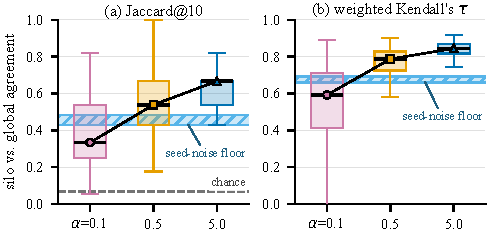
\includegraphics[width=\columnwidth]{figs/fig_agreement_alpha.pdf}
\caption{Silo-versus-global explanation agreement by $\alpha$ (eligible rows; box = IQR,
line = median). Hatched band: centralized-seed instability floor. Dotted line: chance
Jaccard@10. IQRs computed for this paper from agreement\_metrics.csv
(paper/figs/derived\_values.json).}
\label{fig:agree}
\end{figure}

Silo size and label skew are not independent here: a silo's size is the sum of its
Dirichlet shares, so small silos are also skewed ones. We first used label entropy as
the skew covariate, as planned. Its link with agreement did not survive conditioning on
log size: at $\alpha=0.5$ the partial correlation changed sign ($r=+0.23$ and $+0.13$ % src: docs/contribution_a_results.md
for Jaccard@10 and $\tau$, $n=30$). We then substituted KL divergence from the global % src: docs/contribution_a_results.md
label distribution. After conditioning on log size it still predicts agreement: partial
$r=-0.57$ at $\alpha=0.1$ ($n=29$) and $r=-0.82$ and $-0.87$ at $\alpha=0.5$ ($n=30$). % src: docs/contribution_a_results.md
This narrows the size explanation but stays observational; size-controlled partitions
cannot be built with this partitioner.

SHAP's additivity residual also deserves a check, since a poor reconstruction at small
silos could produce low agreement by itself. Of the 90 final-round silo files, 3 store a % src: PROJECT_INSTRUCTIONS.md
residual larger than the worst one in the validation pool (3.336), and these belong % src: PROJECT_INSTRUCTIONS.md
mostly to $\alpha=0.1$. There, the Spearman correlation between a silo's residual and its % src: PROJECT_INSTRUCTIONS.md
Jaccard@10 is $r=-0.237$ ($n=29$). Dropping the flagged silos under a rule written down % src: PROJECT_INSTRUCTIONS.md
in advance keeps Jaccard@10 at 0.333 and shifts $\tau$ from 0.592 to 0.597. Between % src: PROJECT_INSTRUCTIONS.md
rounds 5 and 20, agreement drifts down at $\alpha=0.1$ and $\alpha=0.5$ even as % src: docs/contribution_a_results.md
validation macro-F1 climbs; we treat this trend as directional, since it used a cheaper
SHAP setting and no test. Per-family results, the parity monitor, FedProx and the
faithfulness checks are in \fullref{app:expl} and \fullref{app:resid}.

\subsection{Trust check}
\label{sec:r-trust}
Of the five statistics, only training loss separates the malicious silos: its Glass's
$\delta$ under attack is 33.8 times its value for the same silos in a clean run at $f=3$, % src: PROJECT_INSTRUCTIONS.md
and 154.3 times at $f=2$. These ratios are seed-42 effect sizes, not cut-offs: a % src: PROJECT_INSTRUCTIONS.md
per-round loss cut-off tuned on seed 42 broke down at seed 1337, where it flagged 0.017 % src: PROJECT_INSTRUCTIONS.md
of poisoned silo-rounds against the 0.483 the agent had logged. The three geometric % src: PROJECT_INSTRUCTIONS.md
statistics show little or no separation, and validation accuracy points the wrong way:
relabelling attack flows as Benign makes a malicious silo look more accurate on a
validation set dominated by Benign traffic.

The classical rules did not find the attackers. Multi-Krum excluded a malicious silo
0\% of the time, against a chance rate of 0.30 at $f=3$; it removed the same large, % src: docs/contribution_b_results.md
Benign-heavy silos in every round, attack or not. Its apparent recovery at $f=2$ % src: PROJECT_INSTRUCTIONS.md; docs/contribution_a_results.md; docs/contribution_b_results.md; data/README.md; docs/preregistration_accuracy.md; docs/efficiency_results.md
(recovery fraction 1.3490) is a compositional artifact: dropping those silos raised the % src: docs/contribution_b_results.md
malicious silos' share of the aggregate while lifting macro-F1 through label balance.
Classical Krum keeps one update of ten each round, so its exclusions are at chance.
Defending when nobody attacks has a price in test macro-F1: Krum $-22.7$\,pp, % src: PROJECT_INSTRUCTIONS.md
Multi-Krum $-4.9$\,pp and trimmed mean $-1.6$\,pp. % src: PROJECT_INSTRUCTIONS.md

ByzAgent flagged the malicious silos in 60 of 60 silo-rounds at seed 42, but the same % src: docs/contribution_b_results.md
silos were flagged at 0.95--1.00 in the clean run, as was a silo that was never % src: docs/contribution_b_results.md
malicious. All four are the lowest-Benign silos at that seed. At seeds 1337 and 2024, % src: PROJECT_INSTRUCTIONS.md; docs/contribution_a_results.md; docs/contribution_b_results.md; data/README.md; docs/preregistration_accuracy.md; docs/efficiency_results.md
where composition is graded rather than bimodal, lift appears where the clean baseline
is low (Fig.~\ref{fig:lift}). Our conclusion for this part of the trust check is:
\begin{quote}\small
``Both effects are present. A real compositional confound saturates some silos' flag
rates independent of any attack; real attack-responsive detection is also present and
becomes visible where silos are not already saturated. Seed 42's apparent null was % src: PROJECT_INSTRUCTIONS.md; docs/contribution_a_results.md; docs/contribution_b_results.md; data/README.md; docs/preregistration_accuracy.md; docs/efficiency_results.md
partly a ceiling artifact of that seed's unusually bimodal composition.''
\end{quote}

\begin{figure}[t]
\centering
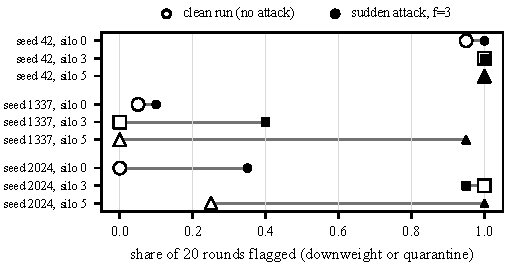
\includegraphics[width=\columnwidth]{figs/fig_byzagent_lift.pdf}
\caption{ByzAgent flag rate for each malicious silo in a clean run (open) and under the
$f=3$ sudden attack (filled). Marker shape: silo 0 (circle), 3 (square), 5 (triangle). % src: PROJECT_INSTRUCTIONS.md; docs/contribution_a_results.md; docs/contribution_b_results.md; data/README.md; docs/preregistration_accuracy.md; docs/efficiency_results.md
Lift is the horizontal distance.}
\label{fig:lift}
\end{figure}

We describe the agent as one that produces decisions plus a rationale of measured
fidelity, and the measurement shows it is partial: its strict citation error rose from 11.7\% (seed 42) to % src: docs/contribution_b_results.md
22.5\% (seeds 1337 and 2024). At those seeds the agent kept citing update norm (in about % src: docs/contribution_b_results.md
59\% of explanations) even though its % src: docs/contribution_b_results.md
correlation with the agent's decisions fell from $+0.419$ to $-0.076$; training loss, % src: docs/contribution_b_results.md
the real signal, stayed under-cited. When given five-round histories, about 35--45\% of % src: PROJECT_INSTRUCTIONS.md
the agent's trend claims contradicted the sequence it was shown. Decisions are
nondeterministic: three repeated calls at round 10 matched exactly in 27 of 30 cases, % src: docs/contribution_b_results.md
and all 30 agreed on trust versus flagged. The rolling-history variant failed its % src: docs/contribution_b_results.md
preregistered test, because a never-malicious silo rose as much as the attackers.
Baselines, the history matrix and the gradual attack are single runs by design. Full
tables are in \fullref{app:trust}.

\subsection{Efficiency}
\label{sec:r-eff}
Table~\ref{tab:eff} summarises the serving and communication measurements. ONNX
Runtime fp32 gives the same predictions as PyTorch on all 143,513 validation rows and is % src: docs/efficiency_results.md
the default serving engine; int8 quantization was dropped after validation macro-F1
fell by 0.1428. Update compression saves bytes exactly, but its effect on accuracy is % src: docs/efficiency_results.md
not detectable at $n=3$. Details are in \fullref{app:eff}. % src: PROJECT_INSTRUCTIONS.md; docs/contribution_a_results.md; docs/contribution_b_results.md; data/README.md; docs/preregistration_accuracy.md; docs/efficiency_results.md

\begin{table}[t]
\centering
\caption{Serving and communication (CPU; one laptop)}
\label{tab:eff}
\footnotesize
\begin{tabularx}{\columnwidth}{@{}>{\raggedright\arraybackslash}Xr@{}}
\toprule
Quantity & Value\\
\midrule
Latency p50 per flow, ONNX fp32 / PyTorch (median, 3 sessions) & 45.7 / 186.5\,$\mu$s\\ % src: PROJECT_INSTRUCTIONS.md
Throughput, batch 1024, ONNX fp32 / PyTorch (rows/s) & 1,071,700 / 1,482,368\\ % src: docs/efficiency_results.md
Traffic per round (fp32, 10 silos, both directions), bytes & 1,587,920\\ % src: PROJECT_INSTRUCTIONS.md
\quad each direction & 793,960\\ % src: PROJECT_INSTRUCTIONS.md
Uplink saving, fp16 / int8 updates & 50.0\% / 74.9\%\\ % src: docs/efficiency_results.md
Best-validation change, fp16 / int8 (mean, 3 seeds) & $-0.0007$ / $-0.0011$\\ % src: docs/efficiency_results.md
Wall time per round, median of 500 rounds & 51.4\,s\\ % src: docs/efficiency_results.md
\bottomrule
\end{tabularx}
\end{table}

% =====================================================================================
\section{Discussion and Limitations}

\emph{What the explanation check supports.} Agreement falls with label skew and sits
well above chance at every $\alpha$. The claim that at $\alpha=0.1$ it is no better than % src: PROJECT_INSTRUCTIONS.md; docs/contribution_a_results.md; docs/contribution_b_results.md; data/README.md; docs/preregistration_accuracy.md; docs/efficiency_results.md
seed noise is directional; the interval touches the floor, and the floor itself rests on
three seed pairs. We used three seeds throughout, so effective sample sizes are closer to
the number of runs than to the number of silo rows. The SHAP sampling in the headline
pipeline was not seeded, the chance level assumes uniform random rankings, and the
faithfulness check (deletion and insertion curves) covers one configuration only. PortScan
generalises genuinely: its test rows sit 23 times further from their nearest training % src: PROJECT_INSTRUCTIONS.md
row than other families do. A suspected near-duplication of Bot and WebAttack rows was
tested and not confirmed. FedProx with $\mu=0.0005$ improved agreement at $\alpha=0.5$ in % src: PROJECT_INSTRUCTIONS.md
all three seeds with flat accuracy, was inconclusive at $\alpha=0.1$ and did nothing at % src: PROJECT_INSTRUCTIONS.md; docs/contribution_a_results.md; docs/contribution_b_results.md; data/README.md; docs/preregistration_accuracy.md; docs/efficiency_results.md
$\alpha=5.0$; we tested no other $\mu$. A drift monitor built on these rankings only % src: PROJECT_INSTRUCTIONS.md; docs/contribution_a_results.md; docs/contribution_b_results.md; data/README.md; docs/preregistration_accuracy.md; docs/efficiency_results.md
works with explanations averaged over at least three draws; single-draw flags were
artifacts.

\emph{What the trust check supports.} The attack is worst-case by construction, and the
attacker-selection rule picks silos on the same composition axis that every detector
here reacts to. Under this partition, a strong attacker drawn from ordinary silos could
not be built, so we cannot say whether the failures are general to these rules or tied
to our selection. The agent's rationale is partly unfaithful, its decisions vary
between calls, and the rolling-history design failed its preregistered test.

% =====================================================================================
\section{Conclusion and Future Work}
On corrected CICIDS2017 split across ten silos, FedAvg holds centralized accuracy at
mild label skew and loses it at strong skew. Explanation agreement between silos and the
global model follows the same direction, and at strong skew it falls to the level that
random seeds produce on their own, a result we report as directional. In a separate
experiment, both the classical robust rules and an LLM trust agent reacted to silo
composition; only the agent also showed attack-responsive flags, and only where silos
were not already saturated. The agent's written reasons were only partly accurate. Next steps include a partitioning design that varies size and skew
independently, seeded multi-draw SHAP for the headline numbers, more seeds for the floor,
attacker selection that does not ride the composition axis, and a check of whether
server momentum changes explanation agreement.

\section*{Acknowledgment}
We thank Prof. Gargi Madala and the School of Computer Science and Engineering,
VIT-AP University, for their guidance and support throughout this project. We also
thank the Canadian Institute for Cybersecurity (CIC) at the University of New Brunswick
for releasing CICIDS2017, and the DistriNet group at KU Leuven for the corrected
version on which every experiment here was run.

\bibliographystyle{IEEEtran}
\bibliography{refs}

% =====================================================================================
\iffullversion
\clearpage
\appendices
% Appendices: the complete record. Input by main.tex only when \iffullversion is true.
% Same rules as the body: every number has a trailing src comment.

\section{Dataset and Cleaning}
\label{app:data}
This appendix gives every data-preparation step with its row counts and supports
Section~IV-A. All counts come from the data-stage decision record \texttt{data/README.md}.

\emph{Lineage.} The flows are the Distrinet CICIDS2017 files, version 4, released with % src: data/README.md; PROJECT_INSTRUCTIONS.md
Liu et al.~\cite{liu2022}. They descend from the corrections of Engelen et
al.~\cite{engelen2021}, which fixed flow construction, feature extraction and labelling
in the original release~\cite{sharafaldin2018} and introduced the ``Attempted'' label for
attack flows that carry no payload. A third correction branch~\cite{lanvin2023} was not
used. The raw data hold 2,099,976 flows in five day files with 91 columns: 7 identifiers, % src: data/README.md
1 label, 1 attempted-category code and 82 numeric candidate features. The attempted % src: data/README.md
code disagrees with the label suffix on none of the rows, so only the suffix is read.

\emph{Attempted flows.} We first planned to fold attempted flows into Benign, as the
dataset authors' own benchmark does. The counts in Table~\ref{tab:attempted} changed that
plan: for several families most flows are attempts, and folding them away would have
emptied Bot and the web attacks. Attempted flows join their parent family under one rule.
As a result, each family's score blends attacks that landed with attempts that did not.

\begin{table}[h]
\centering
\caption{Attempted share of raw families (raw counts)}
\label{tab:attempted}
\footnotesize
\begin{tabular}{@{}lrrr@{}}
\toprule
Raw family & Clean & Attempted & Share\\
\midrule
Web Attack -- XSS & 18 & 655 & 97\%\\ % src: data/README.md
Web Attack -- Brute Force & 73 & 1,292 & 95\%\\ % src: data/README.md
Botnet & 736 & 4,067 & 85\%\\ % src: data/README.md
DoS Slowhttptest & 1,741 & 3,367 & 66\%\\ % src: data/README.md
Infiltration & 36 & 45 & 56\%\\ % src: data/README.md
DoS Slowloris & 3,998 & 1,708 & 30\%\\ % src: data/README.md
DoS Hulk & 158,449 & 581 & 0.4\%\\ % src: data/README.md
\bottomrule
\end{tabular}
\end{table}

\emph{Family mapping.} Fourteen raw labels map to nine classes (Table~\ref{tab:familymap}). % src: data/README.md
The 67,072 ``Infiltration -- Portscan'' flows go to PortScan: they are the internal scan % src: data/README.md
phase of the infiltration scenario and their features are those of a port scan. Routing
them to Infiltration would have made a class that is almost entirely scan traffic, and
every Infiltration explanation would in fact explain a scan. The cost is that
Infiltration shrinks to 66 flows. % src: data/README.md

\begin{table}[h]
\centering
\caption{Raw labels folded into each family}
\label{tab:familymap}
\footnotesize
\begin{tabularx}{\columnwidth}{@{}lX@{}}
\toprule
Family & Raw labels (attempted variants included)\\
\midrule
Benign & BENIGN\\
DoS & DoS Hulk, GoldenEye, Slowloris, Slowhttptest\\
DDoS & DDoS\\
PortScan & Portscan, Infiltration -- Portscan\\
BruteForce & FTP-Patator, SSH-Patator\\
WebAttack & Web Attack Brute Force, XSS, SQL Injection\\
Bot & Botnet\\
Infiltration & Infiltration\\
Heartbleed & Heartbleed\\
\bottomrule
\end{tabularx}
\end{table}

\emph{Cleaning.} The order is load, family mapping, non-finite values, conflicts,
duplicates (Table~\ref{tab:clean}). Five flows with zero duration produce infinite rates % src: data/README.md
and are dropped. The ICMP type and code columns hold $-1$ for non-ICMP flows; this is a % src: data/README.md; PROJECT_INSTRUCTIONS.md
sentinel, not corruption. Groups of identical feature vectors that carry more than one
family cannot be learned and are dropped whole: 43,890 rows in 756 Benign/PortScan % src: data/README.md
groups and 115 rows in 15 Bot/Infiltration groups. Even after correction, then, about % src: data/README.md
forty-four thousand flows cannot be told apart from benign traffic in this feature
space, a ceiling no model can pass. Conflicts are keyed on the family; an earlier
version keyed them on the raw label and silently deleted 58,307 learnable rows. % src: data/README.md

\begin{table}[h]
\centering
\caption{Cleaning steps}
\label{tab:clean}
\footnotesize
\begin{tabular}{@{}lr@{}}
\toprule
Stage & Rows\\
\midrule
Raw flows & 2,099,976\\ % src: data/README.md
Non-finite values removed & $-5$\\ % src: data/README.md
Family conflicts removed & $-44,005$\\ % src: data/README.md
Cross-day duplicates removed & $-142,464$\\ % src: data/README.md
Retained (8.88\% dropped) & 1,913,502\\ % src: data/README.md
\bottomrule
\end{tabular}
\end{table}

\emph{Duplicates.} Before cleaning, 18.3\% of rows are exact copies of another row, and % src: data/README.md
nearly all of them are scan or bot flows: duplicate groups hold 99.2\% of the Portscan % src: data/README.md
rows and 95.0\% of the Infiltration--Portscan rows. % src: data/README.md
Once ports and addresses are removed, many distinct probes collapse to
one vector, so same-day repeats are kept. Only groups that span more than one day file
are removed, since those match the capture-overlap problems reported for this dataset.
Duplicates are keyed on the raw label (provenance), conflicts on the family (target);
keying duplicates on the family once deleted 58,228 rows that were distinct events. % src: data/README.md

\emph{Near-constant features.} Eight of the 82 features have one value in at least % src: data/README.md
99.9\% of rows, but none is constant, so all 82 are kept. % src: data/README.md

\emph{Floor and split.} Families below 1,000 flows stay in the data but leave the % src: data/README.md
headline metric. Table~\ref{tab:families} gives the final distribution and the split.
Even after cleaning, 213,752 rows have at least one identical twin, and the 1,913,502 % src: data/README.md
rows contain only 1,714,074 distinct vectors. % src: data/README.md
The split therefore treats each distinct vector as a group
(stratified group k-fold), checks that no vector appears on both sides, and raises if
one does. All seven headline families land at exactly 25.0\% test share. % src: data/README.md

\begin{table}[h]
\centering
\caption{Families after cleaning and the group-aware split}
\label{tab:families}
\footnotesize
\begin{tabular}{@{}lrrrr@{}}
\toprule
Family & Flows & Train & Test & Test \%\\
\midrule
Benign & 1,440,899 & 1,080,674 & 360,225 & 25.0\\ % src: data/README.md
PortScan & 186,160 & 139,620 & 46,540 & 25.0\\ % src: data/README.md
DoS & 177,491 & 133,118 & 44,373 & 25.0\\ % src: data/README.md
DDoS & 95,144 & 71,358 & 23,786 & 25.0\\ % src: data/README.md
BruteForce & 6,972 & 5,229 & 1,743 & 25.0\\ % src: data/README.md
Bot & 4,703 & 3,527 & 1,176 & 25.0\\ % src: data/README.md
WebAttack & 2,056 & 1,542 & 514 & 25.0\\ % src: data/README.md
Infiltration$^\dagger$ & 66 & 50 & 16 & 24.2\\ % src: data/README.md
Heartbleed$^\dagger$ & 11 & 8 & 3 & 27.3\\ % src: data/README.md
\midrule
Total & 1,913,502 & 1,435,126 & 478,376 & 25.0\\ % src: data/README.md
\bottomrule
\multicolumn{5}{@{}l}{\scriptsize $^\dagger$below the 1,000-flow floor; per class only.}\\ % src: data/README.md
\end{tabular}
\end{table}

\emph{Imbalance.} Benign is 75\% of the data. We use class-weighted loss rather than % src: data/README.md
SMOTE: interpolation would have to run per silo, where minority classes are often a
handful of rows at $\alpha=0.1$; flow features are linked by construction (rate equals % src: data/README.md; PROJECT_INSTRUCTIONS.md
bytes over duration); and synthetic rows would enter the explanation comparison.

\emph{Partitions.} Proportions are applied by cutting each family's shuffled index list
at cumulative boundaries, so shares are exact rather than multinomial draws.
Table~\ref{tab:emptycells} shows the measured heterogeneity. Averaged over families, the
silo that receives most of a family gets 0.694 of it at $\alpha=0.1$, 0.372 at $\alpha=0.5$ and 0.177 at % src: data/README.md
$\alpha=5.0$ (uniform: 0.100). Silo sizes are very uneven at $\alpha=0.1$; the largest % src: data/README.md
silo holds 636,676 rows ($\alpha=0.1$, seed 42, silo 2). Heartbleed, with 8 training % src: results/inspection/silo_size_vs_agreement.csv
flows, cannot fill ten silos, so some cells are empty even at $\alpha=5.0$. The manifest % src: data/README.md
stores a SHA256 hash of each assignment array, not of file contents; a test showed it
catches a single flipped entry among 1.4 million. % src: data/README.md

\begin{table}[h]
\centering
\caption{Empty (silo, family) cells out of 90 per partition} % src: data/README.md; PROJECT_INSTRUCTIONS.md
\label{tab:emptycells}
\footnotesize
\begin{tabular}{@{}lrrr@{}}
\toprule
$\alpha$ & seed 42 & seed 1337 & seed 2024\\ % src: data/README.md; PROJECT_INSTRUCTIONS.md
\midrule
0.1 & 38 & 29 & 31\\ % src: data/README.md
0.5 & 7 & 10 & 8\\ % src: data/README.md
5.0 & 3 & 2 & 2\\ % src: data/README.md
\bottomrule
\end{tabular}
\end{table}

\emph{Leakage controls.} Scalers are fit per silo on training rows; deduplication runs
before partitioning; the split is verified group-aware; partitions are hash-checked at
load; SHAP backgrounds come from each client's training partition; the floor exclusions
were decided once from pooled counts.

% -------------------------------------------------------------------------------------
\section{Model and Training Choices}
\label{app:model}
This appendix gives the pilot runs behind Table~\ref{tab:locked} and the provenance of
each locked choice, supporting Section~IV-B. Pilots are centralized runs ranked on
validation macro-F1 over the seven headline classes.

\begin{table}[h]
\centering
\caption{Centralized pilots: validation macro-F1 (7 classes)} % src: configs/model.yaml; docs/test_set_exposure_audit.md; PROJECT_INSTRUCTIONS.md
\label{tab:pilots}
\footnotesize
\begin{tabular}{@{}llr@{}}
\toprule
Pilot & Arm & Val\\
\midrule
Scaler & standard & 0.9941\\ % src: results/pilots/scaler_comparison.csv
 & robust & 0.9195\\ % src: results/pilots/scaler_comparison.csv
 & robust, clipped & 0.9232\\ % src: results/pilots/scaler_comparison.csv
Class weights & none & 0.9899\\ % src: results/pilots/weights_comparison.csv
 & inverse sqrt & 0.9741\\ % src: results/pilots/weights_comparison.csv
 & effective number, $\beta=0.999$ & 0.9941\\ % src: results/pilots/weights_comparison.csv
 & effective number, $\beta=0.9999$ & 0.9898\\ % src: results/pilots/weights_comparison.csv; docs/handbook/XFed_Team_Handbook.md
 & effective number, $\beta=0.99999$ & 0.9617\\ % src: results/pilots/weights_comparison.csv; configs/model.yaml
Architecture & [128, 64], dropout 0.1 & 0.9939\\ % src: results/pilots/architecture_comparison.csv
 & [128, 64], dropout 0.3 & 0.9931\\ % src: results/pilots/architecture_comparison.csv; configs/model.yaml
 & [256, 128], dropout 0.1 & 0.9912\\ % src: results/pilots/architecture_comparison.csv
 & [256, 128], dropout 0.3 & 0.9878\\ % src: results/pilots/architecture_comparison.csv; configs/model.yaml
 & [512, 256, 128], dropout 0.1 & 0.9936\\ % src: results/pilots/architecture_comparison.csv
 & [512, 256, 128], dropout 0.3 & 0.9938\\ % src: results/pilots/architecture_comparison.csv; configs/model.yaml
\bottomrule
\end{tabular}
\end{table}

The robust scalers fail because 28 of the 82 features have zero interquartile range, % src: PROJECT_INSTRUCTIONS.md
which leaves them unscaled or degenerate. Among architectures the top four arms lie
within 0.0008 on validation, so the smallest, [128, 64] with dropout 0.1, was kept; it % src: docs/test_set_exposure_audit.md
has 19,849 parameters. LayerNorm replaces BatchNorm because running batch statistics are % src: docs/efficiency_results.md
per-silo quantities that FedAvg would average into meaningless values. Local training uses
AdamW (learning rate $10^{-3}$, weight decay $10^{-4}$, batch 1024); centralized runs % src: configs/model.yaml
use up to 50 epochs with early stopping on validation macro-F1 (patience 5) and halve % src: configs/model.yaml
the learning rate on plateaus (patience 3). The validation set is 10\% of the training % src: configs/model.yaml
pool, drawn with seed 42 and held out of every silo. % src: configs/model.yaml

\emph{Provenance.} For three choices, our first written rationale quoted test-set
scores. Table~\ref{tab:provenance} repeats each comparison on validation, and the same
value wins every time. FedProx $\mu=0.01$ collapsed at $\alpha=0.5$, seed 42 (validation macro-F1 % src: docs/test_set_exposure_audit.md
0.7114), which is why $\mu=0.0005$ was carried forward. % src: docs/test_set_exposure_audit.md

\begin{table*}[t]
\centering
\caption{Provenance of locked choices first justified with test numbers}
\label{tab:provenance}
\footnotesize
\begin{tabularx}{\textwidth}{@{}lXX@{}}
\toprule
Choice & Recorded rationale (test) & Validation re-check\\
\midrule
3 local epochs & round-20 test score of \texttt{fedavg\_a0.5\_s42}: macro-F1 0.9747, WebAttack recall 0.9436 & 3 epochs beat 1 at $\alpha=0.5$ in every seed: 0.9760 vs 0.8644, 0.9871 vs 0.8654, 0.8644 vs 0.8508; mean 0.9425 vs 0.8602\\ % src: docs/test_set_exposure_audit.md
FedProx $\mu=0.0005$ & test 0.9794 vs FedAvg 0.9753 ($\alpha=0.5$, s42); $\mu=0.01$: 0.7119 & val 0.9787 vs FedAvg 0.9760; $\mu=0.01$: 0.7114\\ % src: docs/test_set_exposure_audit.md
StandardScaler & test: standard 0.9924, robust-clipped 0.9228, robust 0.9179 & val: standard 0.9941 (best arm)\\ % src: docs/test_set_exposure_audit.md
Class weights $\beta=0.999$ & val 0.9941 and test 0.9924 both cited & best arm on validation\\ % src: docs/test_set_exposure_audit.md
Architecture, dropout & validation only & best arm on validation (0.9939)\\ % src: docs/test_set_exposure_audit.md
\bottomrule
\end{tabularx}
\end{table*}

% -------------------------------------------------------------------------------------
\section{Federated Accuracy, Full}
\label{app:fedacc}
This appendix lists every FedAvg run and the centralized baselines per seed, supporting
Section~VI-A. Test values are single evaluations of validation-selected checkpoints.

\begin{table}[h]
\centering
\caption{FedAvg runs: best round by validation, its validation and test macro-F1, and the round-20 validation score} % src: results/federated/round_lottery_val.csv; PROJECT_INSTRUCTIONS.md; docs/contribution_a_results.md
\label{tab:fedruns}
\footnotesize
\setlength{\tabcolsep}{3.5pt}
\begin{tabular}{@{}llrrrrr@{}}
\toprule
$\alpha$ & Seed & Best rd & Val & Test & Val rd 20 & Gap\\ % src: results/federated/round_lottery_val.csv; PROJECT_INSTRUCTIONS.md; docs/contribution_a_results.md
\midrule
0.1 & 42 & 20 & 0.5440 & 0.5426 & 0.5440 & 0.0000\\ % src: results/federated/round_lottery_val.csv; results/inspection/best_rounds_manifest.json
0.1 & 1337 & 16 & 0.4551 & 0.4481 & 0.4181 & 0.0370\\ % src: results/federated/round_lottery_val.csv; results/inspection/best_rounds_manifest.json
0.1 & 2024 & 16 & 0.5694 & 0.5572 & 0.5565 & 0.0129\\ % src: results/federated/round_lottery_val.csv; results/inspection/best_rounds_manifest.json
0.5 & 42 & 18 & 0.9760 & 0.9753 & 0.9745 & 0.0014\\ % src: results/federated/round_lottery_val.csv; results/inspection/best_rounds_manifest.json
0.5 & 1337 & 11 & 0.9871 & 0.9866 & 0.8699 & 0.1172\\ % src: results/federated/round_lottery_val.csv; results/inspection/best_rounds_manifest.json
0.5 & 2024 & 17 & 0.8644 & 0.8605 & 0.8492 & 0.0152\\ % src: results/federated/round_lottery_val.csv; results/inspection/best_rounds_manifest.json
5.0 & 42 & 18 & 0.9898 & 0.9900 & 0.8713 & 0.1184\\ % src: results/federated/round_lottery_val.csv; results/inspection/best_rounds_manifest.json
5.0 & 1337 & 18 & 0.9898 & 0.9905 & 0.9866 & 0.0032\\ % src: results/federated/round_lottery_val.csv; results/inspection/best_rounds_manifest.json
5.0 & 2024 & 20 & 0.9913 & 0.9889 & 0.9913 & 0.0000\\ % src: results/federated/round_lottery_val.csv; results/inspection/best_rounds_manifest.json
\bottomrule
\end{tabular}
\end{table}

Table~\ref{tab:fedruns} is the round lottery on validation. Best and round-20 checkpoints % src: results/federated/round_lottery_val.csv; PROJECT_INSTRUCTIONS.md; docs/contribution_a_results.md
differ by up to 0.118 (rounded from 0.1184, $\alpha=5.0$, seed 42), so selecting on % src: PROJECT_INSTRUCTIONS.md; results/federated/round_lottery_val.csv
validation is required. Test values for each run are from
\texttt{results/inspection/best\_rounds\_manifest.json}. An earlier version of this
comparison used test scores of the unselected round-20 checkpoints (maximum 0.1199); it % src: docs/contribution_a_results.md
is superseded. Fig.~\ref{fig:valcurves} shows all nine validation curves.

\begin{figure*}[t]
\centering
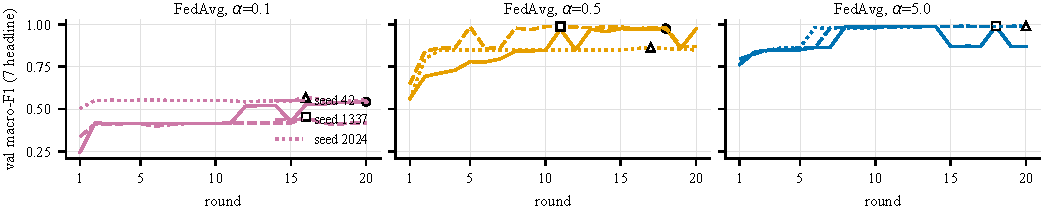
\includegraphics[width=\textwidth]{figs/fig_val_curves.pdf}
\caption{Validation macro-F1 per round for the nine FedAvg runs; open markers show the
best-by-validation round.}
\label{fig:valcurves}
\end{figure*}

\begin{table}[h]
\centering
\caption{Centralized references per seed (test macro-F1, 7 classes; validation in brackets)} % src: results/federated/round_lottery_val.csv; PROJECT_INSTRUCTIONS.md; docs/contribution_a_results.md
\label{tab:centralseed}
\footnotesize
\begin{tabular}{@{}lrr@{}}
\toprule
Seed & Centralized MLP & XGBoost\\
\midrule
42 & 0.9931 [0.9947] & 0.9947 [0.9962]\\ % src: results/centralized/baseline_s42/metrics.json; results/xgboost/xgb_s42/metrics.json; PROJECT_INSTRUCTIONS.md
1337 & 0.9886 [0.9942] & 0.9946 [0.9967]\\ % src: results/centralized/baseline_s1337/metrics.json; results/xgboost/xgb_s1337/metrics.json; PROJECT_INSTRUCTIONS.md
2024 & 0.9884 [0.9946] & 0.9945 [0.9953]\\ % src: results/centralized/baseline_s2024/metrics.json; results/xgboost/xgb_s2024/metrics.json; PROJECT_INSTRUCTIONS.md
Mean $\pm$ std & 0.9900 $\pm$ 0.0022 & 0.9946 $\pm$ 0.0001\\ % src: PROJECT_INSTRUCTIONS.md
\bottomrule
\end{tabular}
\end{table}

The XGBoost values in Table~\ref{tab:centralseed} come from each seed's
\texttt{metrics.json} under \texttt{results/xgboost/}.
Table~\ref{tab:perclass} gives per-class test F1, including the two classes below the
floor. Under FedAvg at $\alpha=0.1$, Bot and WebAttack are almost never detected, and % src: results/federated/round_lottery_val.csv; PROJECT_INSTRUCTIONS.md; docs/contribution_a_results.md
BruteForce, DoS and PortScan swing widely between seeds.

\begin{table*}[t]
\centering
\caption{Per-class test F1 (mean over 3 seeds; FedAvg also shows std). Infiltration and Heartbleed are per class only.} % src: results/federated/round_lottery_val.csv; PROJECT_INSTRUCTIONS.md; docs/contribution_a_results.md
\label{tab:perclass}
\footnotesize
\begin{tabular}{@{}lrrrrr@{}}
\toprule
Class & FedAvg $\alpha=0.1$ & FedAvg $\alpha=0.5$ & FedAvg $\alpha=5.0$ & Centralized MLP & XGBoost\\ % src: results/federated/round_lottery_val.csv; PROJECT_INSTRUCTIONS.md; docs/contribution_a_results.md
\midrule
Benign & 0.9449 $\pm$ 0.0130 & 0.9984 $\pm$ 0.0004 & 0.9993 $\pm$ 0.0000 & 0.9973 & 0.9996\\ % src: results/aggregated/federated_per_family.csv; results/aggregated/centralized_per_family.csv; results/aggregated/xgboost_per_family.csv
Bot & 0.1253 $\pm$ 0.1003 & 0.9404 $\pm$ 0.0410 & 0.9696 $\pm$ 0.0012 & 0.9733 & 0.9804\\ % src: results/aggregated/federated_per_family.csv; results/aggregated/centralized_per_family.csv; results/aggregated/xgboost_per_family.csv
BruteForce & 0.5730 $\pm$ 0.4182 & 0.9929 $\pm$ 0.0023 & 0.9954 $\pm$ 0.0002 & 0.9972 & 0.9978\\ % src: results/aggregated/federated_per_family.csv; results/aggregated/centralized_per_family.csv; results/aggregated/xgboost_per_family.csv
DDoS & 0.9976 $\pm$ 0.0018 & 0.9998 $\pm$ 0.0001 & 0.9999 $\pm$ 0.0001 & 1.0000 & 1.0000\\ % src: results/aggregated/federated_per_family.csv; results/aggregated/centralized_per_family.csv; results/aggregated/xgboost_per_family.csv
DoS & 0.6025 $\pm$ 0.4308 & 0.9947 $\pm$ 0.0047 & 0.9979 $\pm$ 0.0000 & 0.9981 & 0.9987\\ % src: results/aggregated/federated_per_family.csv; results/aggregated/centralized_per_family.csv; results/aggregated/xgboost_per_family.csv
PortScan & 0.3197 $\pm$ 0.4521 & 0.9965 $\pm$ 0.0005 & 0.9974 $\pm$ 0.0000 & 0.9813 & 0.9987\\ % src: results/aggregated/federated_per_family.csv; results/aggregated/centralized_per_family.csv; results/aggregated/xgboost_per_family.csv
WebAttack & 0.0490 $\pm$ 0.0693 & 0.6627 $\pm$ 0.4207 & 0.9691 $\pm$ 0.0058 & 0.9831 & 0.9870\\ % src: results/aggregated/federated_per_family.csv; results/aggregated/centralized_per_family.csv; results/aggregated/xgboost_per_family.csv
Infiltration & 0.0000 $\pm$ 0.0000 & 0.3767 $\pm$ 0.0669 & 0.4362 $\pm$ 0.0502 & 0.7954 & 0.8148\\ % src: results/aggregated/federated_per_family.csv; results/aggregated/centralized_per_family.csv; results/aggregated/xgboost_per_family.csv
Heartbleed & 0.3333 $\pm$ 0.4714 & 0.6000 $\pm$ 0.4320 & 0.9524 $\pm$ 0.0673 & 1.0000 & 1.0000\\ % src: results/aggregated/federated_per_family.csv; results/aggregated/centralized_per_family.csv; results/aggregated/xgboost_per_family.csv
\bottomrule
\end{tabular}
\end{table*}

The centralized and XGBoost per-class columns are from
\texttt{results/aggregated/centralized\_per\_family.csv} and
\texttt{xgboost\_per\_family.csv}. With every class counted, centralized macro-F1 is
0.9695 and XGBoost 0.9752 (means over seeds). % src: results/aggregated/centralized_headline.csv; results/aggregated/xgboost_headline.csv

% -------------------------------------------------------------------------------------
\section{Explanation Check, Full}
\label{app:expl}
This appendix gives every agreement result, the reference lines, the supporting
diagnostics and the negative checks, supporting Section~VI-B. Unless stated, agreement
is the median over eligible rows (silos with at least 400 training rows; families with % src: docs/contribution_a_results.md
at least 20 rows in the silo). % src: docs/contribution_a_results.md
Two measurement choices shape every number here. Each comparison uses the attribution
vector of the row's true class, so disagreement about the prediction itself is left out
by design; a version anchored on each model's own predicted class would answer a
different question and would need its own eligibility rules. And, as with any
perturbation-based explainer, SHAP's stand-in for a ``missing'' feature is a background
average, which is not a real network flow.

\subsection{Agreement by $\alpha$ and by family}
Table~\ref{tab:agree_alpha} gives the median and interquartile range of each metric per
$\alpha$, and Table~\ref{tab:agree_family} breaks Jaccard@10 and $\tau$ down by family.
IQRs computed for this paper from agreement\_metrics.csv
(\texttt{paper/figs/derived\_values.json}), by \texttt{paper/figs/make\_figs.py}; the
medians reproduce the published ones.

\begin{table*}[t]
\centering
\caption{Agreement per $\alpha$: median [Q1, Q3] over eligible rows}
\label{tab:agree_alpha}
\footnotesize
\setlength{\tabcolsep}{3pt}
\begin{tabular}{@{}lccc@{}}
\toprule
 & $\alpha=0.1$ & $\alpha=0.5$ & $\alpha=5.0$\\ % src: docs/contribution_a_results.md; docs/measurement_protocol.md; PROJECT_INSTRUCTIONS.md
\midrule
Eligible / all rows & 220 / 406 & 388 / 420 & 420 / 420\\ % src: site/public/data/agreement_by_alpha.json
Jaccard@5 & 0.250 & 0.429 & 0.667\\ % src: site/public/data/agreement_by_alpha.json
Jaccard@10 & 0.333 [0.250, 0.538] & 0.538 [0.429, 0.667] & 0.667 [0.538, 0.667]\\ % src: paper/figs/derived_values.json
Jaccard@20 & 0.379 & 0.600 & 0.667\\ % src: site/public/data/agreement_by_alpha.json
Weighted $\tau$ & 0.592 [0.413, 0.712] & 0.787 [0.725, 0.827] & 0.844 [0.818, 0.868]\\ % src: paper/figs/derived_values.json
\bottomrule
\end{tabular}
\end{table*}

\begin{table*}[t]
\centering
\caption{Agreement by family: median [Q1, Q3] over eligible rows ($n$ = eligible rows)}
\label{tab:agree_family}
\footnotesize
\setlength{\tabcolsep}{3pt}
\begin{tabular}{@{}l rcc rcc rcc@{}}
\toprule
 & \multicolumn{3}{c}{$\alpha=0.1$} & \multicolumn{3}{c}{$\alpha=0.5$} & \multicolumn{3}{c}{$\alpha=5.0$}\\ % src: docs/contribution_a_results.md; docs/measurement_protocol.md; PROJECT_INSTRUCTIONS.md
\cmidrule(lr){2-4}\cmidrule(lr){5-7}\cmidrule(l){8-10}
Family & $n$ & Jaccard@10 & $\tau$ & $n$ & Jaccard@10 & $\tau$ & $n$ & Jaccard@10 & $\tau$\\
\midrule
Benign & 46 & 0.333 [0.250, 0.538] & 0.649 [0.532, 0.716] & 56 & 0.538 [0.429, 0.667] & 0.772 [0.737, 0.806] & 60 & 0.667 [0.538, 0.667] & 0.830 [0.794, 0.851]\\ % src: paper/figs/derived_values.json
Bot & 26 & 0.250 [0.176, 0.405] & 0.560 [0.347, 0.696] & 54 & 0.484 [0.429, 0.538] & 0.751 [0.698, 0.795] & 60 & 0.538 [0.429, 0.667] & 0.818 [0.789, 0.845]\\ % src: paper/figs/derived_values.json
BruteForce & 28 & 0.333 [0.250, 0.538] & 0.596 [0.403, 0.696] & 52 & 0.538 [0.429, 0.667] & 0.803 [0.692, 0.842] & 60 & 0.667 [0.538, 0.667] & 0.841 [0.811, 0.848]\\ % src: paper/figs/derived_values.json
DDoS & 34 & 0.381 [0.250, 0.538] & 0.620 [0.464, 0.736] & 60 & 0.603 [0.538, 0.667] & 0.808 [0.773, 0.839] & 60 & 0.818 [0.667, 0.818] & 0.858 [0.842, 0.881]\\ % src: paper/figs/derived_values.json
DoS & 38 & 0.381 [0.250, 0.538] & 0.688 [0.549, 0.740] & 60 & 0.538 [0.429, 0.667] & 0.819 [0.783, 0.855] & 60 & 0.667 [0.667, 0.818] & 0.876 [0.856, 0.887]\\ % src: paper/figs/derived_values.json
PortScan & 32 & 0.250 [0.176, 0.429] & 0.519 [0.354, 0.632] & 58 & 0.538 [0.538, 0.667] & 0.788 [0.740, 0.814] & 60 & 0.667 [0.538, 0.818] & 0.861 [0.839, 0.881]\\ % src: paper/figs/derived_values.json
WebAttack & 16 & 0.292 [0.250, 0.333] & 0.416 [0.335, 0.583] & 48 & 0.538 [0.429, 0.667] & 0.769 [0.637, 0.798] & 60 & 0.538 [0.538, 0.667] & 0.823 [0.807, 0.843]\\ % src: paper/figs/derived_values.json
\bottomrule
\end{tabular}
\end{table*}

\subsection{Reference lines and uncertainty}
Chance Jaccard@$k$ is the ratio of the expected intersection $k^2/n$ to the expected
union $2k-k^2/n$ for two independent uniform $k$-subsets of $n$ items; with $k=10$ and % src: docs/contribution_a_results.md; docs/measurement_protocol.md; PROJECT_INSTRUCTIONS.md
$n=82$ it is 0.065. The instability floor uses three centralized models (seeds 42, 1337, % src: docs/measurement_protocol.md
2024) explained with the same 14 rows, 4000 samples and class-stratified 200-row % src: docs/measurement_protocol.md
background construction as the federated pipeline. Table~\ref{tab:floor} gives each seed
pair; the floor is the median of the pair medians, with their range.

\begin{table}[h]
\centering
\caption{Centralized-seed instability floor per seed pair (median over 14 rows)} % src: docs/contribution_a_results.md; docs/measurement_protocol.md; PROJECT_INSTRUCTIONS.md
\label{tab:floor}
\footnotesize
\begin{tabular}{@{}lrr@{}}
\toprule
Seed pair & Jaccard@10 & Weighted $\tau$\\
\midrule
42--1337 & 0.484 & 0.660\\ % src: site/public/data/headline.json
42--2024 & 0.429 & 0.690\\ % src: site/public/data/headline.json
1337--2024 & 0.429 & 0.663\\ % src: site/public/data/headline.json
Floor: median [range] & 0.429 [0.429, 0.484] & 0.663 [0.660, 0.690]\\ % src: site/public/data/headline.json
\bottomrule
\end{tabular}
\end{table}

The cluster bootstrap resamples (seed, silo) clusters with replacement, 10,000 times % src: site/public/data/ci.json
(29 clusters at $\alpha=0.1$), and takes the median of all rows in each resample. At % src: site/public/data/ci.json
$\alpha=0.1$ the 95\% percentile interval is [0.250, 0.429] for Jaccard@10 and % src: site/public/data/ci.json
[0.541, 0.661] for weighted $\tau$. The Jaccard interval overlaps the floor range, so the % src: site/public/data/ci.json
below-floor reading at $\alpha=0.1$ is directional, not significant. An interval was % src: docs/contribution_a_results.md; docs/measurement_protocol.md; PROJECT_INSTRUCTIONS.md
computed only for $\alpha=0.1$; none exists on disk for the other two levels. % src: docs/contribution_a_results.md; docs/measurement_protocol.md; PROJECT_INSTRUCTIONS.md

\subsection{Size and label skew}
Under the partitioner, a silo's size is $\sum_k N_k\,p_k[i]$, a function of the same
draw that sets its skew. A raw size correlation therefore restates the skew effect:
silo size and Jaccard@10 correlate at $r=+0.46$ at $\alpha=0.1$ and $r=+0.07$ at % src: docs/contribution_a_results.md
$\alpha=5.0$. Label entropy over the nine classes was the covariate fixed in advance. Its % src: docs/contribution_a_results.md; docs/measurement_protocol.md; PROJECT_INSTRUCTIONS.md
zero-order correlation with agreement at $\alpha=0.5$ was weak and negative, and after % src: docs/contribution_a_results.md; docs/measurement_protocol.md; PROJECT_INSTRUCTIONS.md
conditioning on log size its partial correlation changed sign, so it was dropped. We
then tried the KL divergence between each silo's label mix and the global one
(Table~\ref{tab:kl}).
Fig.~\ref{fig:kl} shows the per-silo values. A design that varies size and skew
independently is not possible with this partitioner, so the analysis stays observational.

\begin{table}[h]
\centering
\caption{Correlation of a skew covariate with agreement after conditioning on log silo size ($r$ and $n$ only)}
\label{tab:kl}
\footnotesize
\begin{tabular}{@{}llllr@{}}
\toprule
Order & Covariate & $\alpha$ & Partial $r$ (J@10 / $\tau$) & $n$\\ % src: docs/contribution_a_results.md; docs/measurement_protocol.md; PROJECT_INSTRUCTIONS.md
\midrule
1st & entropy & 0.5 & $+0.23$ / $+0.13$ & 30\\ % src: docs/contribution_a_results.md
2nd & KL from global & 0.1 & $-0.57$ / -- & 29\\ % src: docs/contribution_a_results.md
2nd & KL from global & 0.5 & $-0.82$ / $-0.87$ & 30\\ % src: docs/contribution_a_results.md
\bottomrule
\end{tabular}
\end{table}

\begin{figure}[h]
\centering
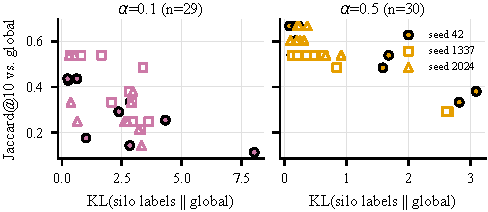
\includegraphics[width=\columnwidth]{figs/fig_kl_scatter.pdf}
\caption{Per-silo KL divergence from the global label mix against Jaccard@10 (final
round). Filled: seed 42; open square and triangle: seeds 1337 and 2024.} % src: docs/contribution_a_results.md; docs/measurement_protocol.md; PROJECT_INSTRUCTIONS.md
\label{fig:kl}
\end{figure}

\subsection{Round-wise agreement}
Agreement was recomputed at rounds 5, 10, 15 and 20 with 1000 SHAP samples, a quarter % src: docs/contribution_a_results.md
of the headline setting, so these values check the shape of convergence and are not
comparable in size with Table~\ref{tab:agree_alpha}. Table~\ref{tab:roundwise} and
Fig.~\ref{fig:roundwise} give the means. From round 5 to 20, Jaccard@10 falls by 0.023 % src: docs/contribution_a_results.md
at $\alpha=0.1$ and 0.029 at $\alpha=0.5$ while validation macro-F1 rises by 0.046 and % src: docs/contribution_a_results.md
0.026; at $\alpha=5.0$ the four Jaccard values span 0.004. No test was run on this % src: docs/contribution_a_results.md
trend; it is directional.

\begin{table}[h]
\centering
\caption{Round-wise means (reduced SHAP fidelity)}
\label{tab:roundwise}
\footnotesize
\setlength{\tabcolsep}{4pt}
\begin{tabular}{@{}llrrrr@{}}
\toprule
Metric & $\alpha$ & Rd 5 & Rd 10 & Rd 15 & Rd 20\\ % src: docs/contribution_a_results.md; docs/measurement_protocol.md; PROJECT_INSTRUCTIONS.md
\midrule
Jaccard@10 & 0.1 & 0.359 & 0.350 & 0.334 & 0.336\\ % src: docs/contribution_a_results.md
 & 0.5 & 0.560 & 0.542 & 0.548 & 0.531\\ % src: docs/contribution_a_results.md
 & 5.0 & 0.640 & 0.641 & 0.642 & 0.644\\ % src: docs/contribution_a_results.md
Weighted $\tau$ & 0.1 & 0.524 & 0.548 & 0.541 & 0.529\\ % src: docs/contribution_a_results.md
 & 0.5 & 0.770 & 0.760 & 0.759 & 0.742\\ % src: docs/contribution_a_results.md
 & 5.0 & 0.830 & 0.828 & 0.822 & 0.830\\ % src: docs/contribution_a_results.md
Val macro-F1 & 0.1 & 0.460 & 0.461 & 0.464 & 0.506\\ % src: docs/contribution_a_results.md
 & 0.5 & 0.872 & 0.895 & 0.937 & 0.898\\ % src: docs/contribution_a_results.md
 & 5.0 & 0.860 & 0.984 & 0.949 & 0.950\\ % src: docs/contribution_a_results.md
\bottomrule
\end{tabular}
\end{table}

\begin{figure}[h]
\centering
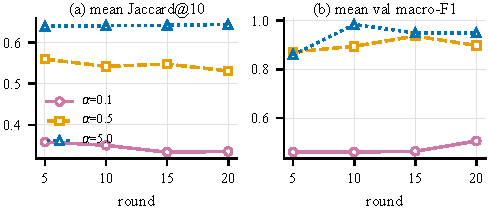
\includegraphics[width=\columnwidth]{figs/fig_round_wise.pdf}
\caption{Round-wise mean Jaccard@10 (a) and validation macro-F1 (b).}
\label{fig:roundwise}
\end{figure}

\subsection{FedProx at $\mu=0.0005$}
FedProx~\cite{li2020fedprox} was run at one value, $\mu=0.0005$, carried forward from an % src: docs/contribution_a_results.md
exploratory run; it was never swept. Table~\ref{tab:fedprox} compares it with FedAvg per
seed using the mean over eligible rows (not the median used elsewhere). At $\alpha=0.5$ % src: docs/contribution_a_results.md; docs/measurement_protocol.md; PROJECT_INSTRUCTIONS.md
Jaccard@10 rises in all three seeds while test macro-F1 moves by small amounts of mixed
sign. At $\alpha=0.1$ agreement and accuracy move together in each seed, so $n=3$ cannot % src: docs/contribution_a_results.md; docs/measurement_protocol.md; PROJECT_INSTRUCTIONS.md
separate an explanation effect from an accuracy effect; we treat it as inconclusive. At
$\alpha=5.0$ there is no consistent change. % src: docs/contribution_a_results.md; docs/measurement_protocol.md; PROJECT_INSTRUCTIONS.md

\begin{table*}[t]
\centering
\caption{FedAvg vs FedProx ($\mu=0.0005$): mean agreement over eligible rows and test macro-F1 per seed} % src: docs/contribution_a_results.md; docs/measurement_protocol.md; PROJECT_INSTRUCTIONS.md
\label{tab:fedprox}
\footnotesize
\begin{tabular}{@{}ll rrr rrr rrr@{}}
\toprule
 & & \multicolumn{3}{c}{Jaccard@10} & \multicolumn{3}{c}{Weighted $\tau$} & \multicolumn{3}{c}{Test macro-F1}\\
\cmidrule(lr){3-5}\cmidrule(lr){6-8}\cmidrule(l){9-11}
$\alpha$ & Seed & FedAvg & FedProx & $\Delta$ & FedAvg & FedProx & $\Delta$ & FedAvg & FedProx & $\Delta$\\
\midrule
0.1 & 42 & 0.3257 & 0.3917 & +0.0660 & 0.5078 & 0.6176 & +0.1098 & 0.5426 & 0.5526 & +0.0100\\ % src: docs/contribution_a_results.md
0.1 & 1337 & 0.3979 & 0.3312 & $-0.0667$ & 0.6147 & 0.5689 & $-0.0458$ & 0.4481 & 0.4202 & $-0.0279$\\ % src: docs/contribution_a_results.md
0.1 & 2024 & 0.3301 & 0.4109 & +0.0808 & 0.5331 & 0.6265 & +0.0934 & 0.5572 & 0.6265 & +0.0693\\ % src: docs/contribution_a_results.md
0.5 & 42 & 0.5444 & 0.5707 & +0.0263 & 0.7545 & 0.7647 & +0.0102 & 0.9753 & 0.9794 & +0.0041\\ % src: docs/contribution_a_results.md
0.5 & 1337 & 0.5096 & 0.5269 & +0.0173 & 0.7318 & 0.7565 & +0.0247 & 0.9866 & 0.9846 & $-0.0020$\\ % src: docs/contribution_a_results.md
0.5 & 2024 & 0.6167 & 0.6209 & +0.0042 & 0.7913 & 0.7904 & $-0.0009$ & 0.8605 & 0.8591 & $-0.0014$\\ % src: docs/contribution_a_results.md
5.0 & 42 & 0.6406 & 0.6441 & +0.0035 & 0.8415 & 0.8396 & $-0.0018$ & 0.9900 & 0.9889 & $-0.0011$\\ % src: docs/contribution_a_results.md
5.0 & 1337 & 0.6688 & 0.6593 & $-0.0095$ & 0.8385 & 0.8330 & $-0.0055$ & 0.9905 & 0.9890 & $-0.0015$\\ % src: docs/contribution_a_results.md
5.0 & 2024 & 0.6269 & 0.6732 & +0.0463 & 0.8373 & 0.8391 & +0.0018 & 0.9889 & 0.9919 & +0.0029\\ % src: docs/contribution_a_results.md
\bottomrule
\end{tabular}
\end{table*}

\subsection{Parity monitor}
The parity monitor turns each silo's top-10 index list into a leave-one-out deviation % src: docs/contribution_a_results.md; docs/measurement_protocol.md; PROJECT_INSTRUCTIONS.md
from the fleet consensus and flags silos whose modified z-score, computed from the
median and the median absolute deviation, exceeds 3.5~\cite{iglewicz1993}. It uses only % src: docs/contribution_a_results.md
what would cross the client-server boundary. Over the full sweep (9 configurations, % src: docs/contribution_a_results.md
4 rounds, 356 rows) it raised 3 flags, all at $\alpha=0.5$, round 5 % src: docs/contribution_a_results.md
(Table~\ref{tab:parity}). Zero flags at $\alpha=0.1$ does not mean the fleet is healthy: % src: docs/contribution_a_results.md; docs/measurement_protocol.md; PROJECT_INSTRUCTIONS.md
at round 5 the median deviation across 29 eligible silos was 0.694, worse than any of % src: docs/contribution_a_results.md
the flagged values, but every silo diverged about equally, so none stood out.

\begin{table}[h]
\centering
\caption{Parity-monitor flags (three-draw average)}
\label{tab:parity}
\footnotesize
\begin{tabular}{@{}lrrr@{}}
\toprule
Run & Seed & Silo & Deviation\\
\midrule
\texttt{fedavg\_a0.5\_s1337} & 1337 & 7 & 0.775\\ % src: docs/contribution_a_results.md
\texttt{fedavg\_a0.5\_s2024} & 2024 & 3 & 0.530\\ % src: docs/contribution_a_results.md
\texttt{fedavg\_a0.5\_s2024} & 2024 & 6 & 0.535\\ % src: docs/contribution_a_results.md
\bottomrule
\end{tabular}
\end{table}

When the monitor still relied on one explainer draw, it flagged two silos of % src: docs/contribution_a_results.md
\texttt{fedavg\_a0.1\_s1337} at round 5 (deviations 0.947 and 0.889); explaining the same % src: docs/contribution_a_results.md
checkpoints again did not reproduce either flag. The cached draw happened to produce many tied deviations, which shrank
that round's median absolute deviation to 0.042, about a third of what fresh draws gave. % src: docs/contribution_a_results.md
The threshold formula was sound; judging it on one draw was not. The monitor now explains
each checkpoint three times with fixed seeds (1001, 2002, 3003), computes each draw's % src: docs/contribution_a_results.md
deviation separately and averages before thresholding.

\subsection{Faithfulness and explainer checks}
Deletion and insertion curves~\cite{petsiuk2018} replace features by the model's
training mean in ranked order. They were run for one configuration ($\alpha=0.5$, seed % src: docs/contribution_a_results.md; docs/measurement_protocol.md; PROJECT_INSTRUCTIONS.md
42) on the global model and three of ten silos (Table~\ref{tab:faith}). Every deletion % src: docs/contribution_a_results.md; docs/measurement_protocol.md; PROJECT_INSTRUCTIONS.md
AUC lies below the matching insertion AUC, which fits attributions that track the
model. There is no agreed threshold for these AUCs, and nothing downstream is gated on
them; this is a spot-check, not a gate.

\begin{table}[h]
\centering
\caption{Deletion (lower is better) and insertion (higher is better) AUC, $\alpha=0.5$, seed 42} % src: docs/contribution_a_results.md; docs/measurement_protocol.md; PROJECT_INSTRUCTIONS.md
\label{tab:faith}
\footnotesize
\begin{tabular}{@{}lrr@{}}
\toprule
Model & Deletion AUC & Insertion AUC\\
\midrule
Global & 0.167 & 0.696\\ % src: docs/contribution_a_results.md
Silo 0 & 0.274 & 0.800\\ % src: docs/contribution_a_results.md
Silo 1 & 0.166 & 0.628\\ % src: docs/contribution_a_results.md
Silo 2 & 0.179 & 0.655\\ % src: docs/contribution_a_results.md
\bottomrule
\end{tabular}
\end{table}

Two further checks test the measurement itself. KernelExplainer and GradientExplainer
on the same models agree at median $\tau=0.730$ and Jaccard@10 0.538 ($n=14$), so the % src: docs/contribution_a_results.md
rankings are not an artifact of the explainer. Replacing per-silo backgrounds with a
common one gives median $\tau=0.807$ and Jaccard@10 0.603 ($n=42$), so disagreement is % src: docs/contribution_a_results.md
not a background artifact. DeepExplainer was rejected after a probe: its additivity error
on this model is 2.43 because of LayerNorm. SHAP on this 19,849-parameter model ran % src: PROJECT_INSTRUCTIONS.md; docs/efficiency_results.md
about 3 times slower on the GPU than on the CPU, so all SHAP work used the CPU. The % src: docs/contribution_a_results.md
Monte Carlo sampling inside GradientExplainer is not seeded in the headline pipeline:
rerunning one global model gave a mean absolute difference of 0.0188 and a maximum of % src: docs/contribution_a_results.md
0.403 between draws. % src: docs/contribution_a_results.md

\subsection{Generalisation and near-duplication}
PortScan is the family whose test rows are genuinely new: their nearest training rows
are 23 times further away than for other families, and its recall is bimodal across % src: PROJECT_INSTRUCTIONS.md
seeds (0.9505, 0.9506, 0.9995). A nearest-neighbour audit found Bot and WebAttack test % src: docs/contribution_a_results.md
rows nearly identical to training rows, which raised a preregistered concern that their
agreement could be inflated. The concern was tested and not confirmed; thin support
(3,527 Bot and 1,542 WebAttack training rows) explains their behaviour better. % src: docs/contribution_a_results.md

\subsection{An open pattern at $\alpha=0.5$}
Three separate analyses single out $\alpha=0.5$: all parity flags occur there, the KL % src: docs/contribution_a_results.md; docs/measurement_protocol.md; PROJECT_INSTRUCTIONS.md
partial correlation is strongest there, and the FedProx agreement gain is clean only
there. We record this as an open pattern and propose no mechanism.

% -------------------------------------------------------------------------------------
\section{SHAP Additivity Residuals}
\label{app:resid}
This appendix gives the additivity residuals of the SHAP values and the sensitivity of
the headline agreement to them, supporting Section~VI-B. For a row $x$, the relative
residual is the largest over classes of $|\sum\mathrm{SHAP}-(f(x)-E[f])|$ divided by the
largest over classes of $|f(x)-E[f]|$.

\emph{Validation pool.} For the served model, 500 validation rows were explained with % src: results/shap/fedavg_a0.5_s42/val_pool_summary.json
4000 samples (Table~\ref{tab:valpool}). Of the 18 rows above 8\%, seven are Bot, four % src: PROJECT_INSTRUCTIONS.md; results/shap/fedavg_a0.5_s42/val_pool_summary.json
Benign and four WebAttack; the worst case, at 21.2\%, is an Infiltration row. A range % src: PROJECT_INSTRUCTIONS.md
of ``3--8\%'' quoted in earlier project notes could not be traced to any file, so we % src: PROJECT_INSTRUCTIONS.md
dropped it. For the 14 test rows the residual cannot be recomputed at all: their saved % src: PROJECT_INSTRUCTIONS.md
SHAP files lack the model outputs it needs.

\begin{table}[h]
\centering
\caption{Additivity residuals on 500 validation rows} % src: PROJECT_INSTRUCTIONS.md; docs/contribution_a_results.md; results/shap/fedavg_a0.5_s42/val_pool_summary.json
\label{tab:valpool}
\footnotesize
\begin{tabular}{@{}lrrr@{}}
\toprule
 & Median & p95 & Max\\ % src: PROJECT_INSTRUCTIONS.md; docs/contribution_a_results.md; results/shap/fedavg_a0.5_s42/val_pool_summary.json
\midrule
Relative & 3.2\% & 7.7\% & 21.2\%\\ % src: PROJECT_INSTRUCTIONS.md
Absolute (logit) & 0.472 & 1.105 & 3.336\\ % src: docs/contribution_a_results.md
\bottomrule
\end{tabular}
\end{table}

\emph{Audit of stored residuals.} A stored value is the worst residual among 14 rows, % src: PROJECT_INSTRUCTIONS.md
which makes any comparison with a single-row maximum rough. Table~\ref{tab:residaudit} % src: PROJECT_INSTRUCTIONS.md; docs/contribution_a_results.md; results/shap/fedavg_a0.5_s42/val_pool_summary.json
counts files above the validation-pool maximum of 3.336. Among final-round FedAvg files, % src: results/inspection/residual_audit_summary.json
4 of 99 exceed it: silos 3 and 9 of $\alpha=0.1$ seed 42, silo 8 of $\alpha=0.1$ seed % src: results/inspection/residual_audit_summary.json
1337 (two of these three silos are the smallest in their run), and the global % src: PROJECT_INSTRUCTIONS.md; docs/contribution_a_results.md; results/shap/fedavg_a0.5_s42/val_pool_summary.json
model of $\alpha=5.0$ seed 1337 (3.500). Stored values range from 0.156 to 15.874. % src: docs/contribution_a_results.md

\begin{table}[h]
\centering
\caption{Stored residual files above 3.336, and Spearman $r$ between silo residual and Jaccard@10 (FedAvg, final round)} % src: PROJECT_INSTRUCTIONS.md; docs/contribution_a_results.md; results/shap/fedavg_a0.5_s42/val_pool_summary.json
\label{tab:residaudit}
\footnotesize
\setlength{\tabcolsep}{2.5pt}
\begin{tabular}{@{}lrrrr@{}}
\toprule
Pass & $\alpha=0.1$ & $\alpha=0.5$ & $\alpha=5.0$ & Silo / global\\ % src: PROJECT_INSTRUCTIONS.md; docs/contribution_a_results.md; results/shap/fedavg_a0.5_s42/val_pool_summary.json
\midrule
FedAvg final & 3/33 & 0/33 & 1/33 & 3/90, 1/9\\ % src: results/inspection/residual_audit_summary.json
FedAvg round-wise & 26/132 & 0/132 & 5/132 & 29/360, 2/36\\ % src: results/inspection/residual_audit_summary.json
FedProx final & 1/33 & 0/33 & 0/33 & 1/90, 0/9\\ % src: results/inspection/residual_audit_summary.json
\midrule
Spearman $r$ ($n$), final & $-0.237$ (29) & 0.202 (30) & 0.11 (30) & \\ % src: results/inspection/residual_audit_summary.json
\bottomrule
\end{tabular}
\end{table}

\emph{Sensitivity.} The exclusion rule was fixed before computing: drop any silo whose
final-round residual exceeds 3.336. At $\alpha=0.1$ the rule takes out two silos that % src: PROJECT_INSTRUCTIONS.md
contribute eligible rows, 8 of the 220; the Jaccard@10 median does not move from 0.333, % src: PROJECT_INSTRUCTIONS.md
and the $\tau$ median goes from 0.592 to 0.597. % src: PROJECT_INSTRUCTIONS.md
Nothing is removed at $\alpha=0.5$ or $5.0$. \emph{Post-hoc, outside the rule:} % src: PROJECT_INSTRUCTIONS.md
if the whole $\alpha=5.0$ seed-1337 run is removed because its global model is flagged, % src: PROJECT_INSTRUCTIONS.md
the $\alpha=5.0$ medians are still 0.667 for Jaccard@10 and 0.844 for $\tau$. % src: PROJECT_INSTRUCTIONS.md

% -------------------------------------------------------------------------------------
\section{Trust Check, Full}
\label{app:trust}
This appendix gives every phase of the trust check, supporting Section~VI-C. Unless
stated, results are for $\alpha=0.5$, seed 42, 10 silos and 20 rounds; Phase 2, the % src: docs/contribution_b_results.md; PROJECT_INSTRUCTIONS.md
Phase 4 matrix and the gradual attack are single runs by design. The attack is a
worst-case, full-knowledge construction throughout. The trust check does not claim that
ByzAgent beats the classical rules; its value is in what it shows about all of them and
in the audit of its stated reasons. A planned benchmarking harness pitting ByzAgent
against the baselines was not built, because both baselines already fail for reasons
such a harness would not add evidence to.

\subsection{Phase 0: attack construction and strength}
The attack flips 40\% of each malicious silo's non-Benign rows to Benign (seed 9001). % src: docs/contribution_b_results.md
Among all $\binom{10}{3}=120$ triples, the attacker set is the one whose weakest % src: docs/contribution_b_results.md
attack family would be most covered if every eligible row were flipped; for
$\{0,3,5\}$ that weakest family is DoS, at 38.60\%. % src: docs/contribution_b_results.md
A secondary $f=2$ condition, $\{0,3\}$, reaches 16.73\%. An % src: docs/contribution_b_results.md
earlier rule that picked size-representative silos $\{0,1,9\}$ reached 13.98\% coverage % src: docs/contribution_b_results.md
with three families under 5\% and was retired as too weak. Logged flips matched the % src: docs/contribution_b_results.md; PROJECT_INSTRUCTIONS.md
expected coverage within one to two percentage points on every family.
Table~\ref{tab:phase0} reports all four statistics; Fig.~\ref{fig:phase0} shows the
curves. The final-five mean drops by 3.7 to 7.7 points and orders correctly by coverage, % src: docs/contribution_b_results.md
while the maximum barely moves: a constant-fraction attack shifts the curve, and the
maximum is insensitive to such a shift. Both statistics are therefore always reported.

\begin{table*}[t]
\centering
\caption{Phase 0: validation macro-F1 over 20 rounds ($\Delta$ vs clean)} % src: docs/contribution_b_results.md; PROJECT_INSTRUCTIONS.md
\label{tab:phase0}
\footnotesize
\setlength{\tabcolsep}{2.5pt}
\begin{tabular}{@{}lrrrr@{}}
\toprule
Statistic & Clean & $\{0,1,9\}$ (retired) & $\{0,3,5\}$, $f=3$ & $\{0,3\}$, $f=2$\\ % src: docs/contribution_b_results.md; PROJECT_INSTRUCTIONS.md
\midrule
Mean & 0.8535 & 0.8180 ($-0.0355$) & 0.8236 ($-0.0299$) & 0.8253 ($-0.0282$)\\ % src: docs/contribution_b_results.md
Median & 0.8487 & 0.8436 ($-0.0051$) & 0.8438 ($-0.0048$) & 0.8489 (+0.0003)\\ % src: docs/contribution_b_results.md
Final-5 mean & 0.9513 & 0.9143 ($-0.0370$) & 0.8746 ($-0.0766$) & 0.8787 ($-0.0726$)\\ % src: docs/contribution_b_results.md
Max & 0.9760 & 0.9710 ($-0.0049$) & 0.9763 (+0.0004) & 0.9867 (+0.0107)\\ % src: docs/contribution_b_results.md
\bottomrule
\end{tabular}
\end{table*}

\begin{figure}[h]
\centering
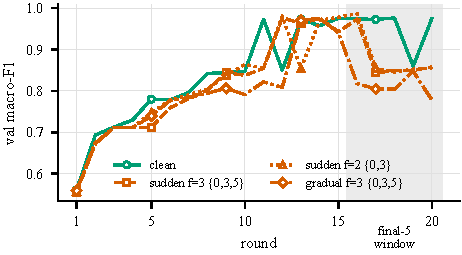
\includegraphics[width=\columnwidth]{figs/fig_phase0_curves.pdf}
\caption{Validation macro-F1 of the clean run and the three $\{0,3,5\}$/$\{0,3\}$ % src: docs/contribution_b_results.md; PROJECT_INSTRUCTIONS.md
poisoned runs at seed 42; shaded: final-five window.} % src: docs/contribution_b_results.md; PROJECT_INSTRUCTIONS.md
\label{fig:phase0}
\end{figure}

\emph{Gradual mode.} The flip fraction ramps as $\min(0.05+0.05(r-1),1)$, reaching 1.0 % src: docs/contribution_b_results.md
at round 20 and equalling the sudden attack's 0.40 at round 8, so rounds 1--8 are the % src: docs/contribution_b_results.md
strength-matched window. In its final five rounds the gradual attack is 2--2.5 times % src: docs/contribution_b_results.md
stronger than the sudden one, so its larger drops in Table~\ref{tab:gradual} reflect a
stronger attack. In rounds 1--8 the per-round gap to the clean run is small and
non-monotonic ($-0.001$ to $-0.041$). % src: docs/contribution_b_results.md

\begin{table}[h]
\centering
\caption{Sudden vs gradual $\{0,3,5\}$ ($\Delta$ vs clean)} % src: docs/contribution_b_results.md; PROJECT_INSTRUCTIONS.md
\label{tab:gradual}
\footnotesize
\begin{tabular}{@{}lrrr@{}}
\toprule
Statistic & Clean & Sudden & Gradual\\
\midrule
Mean & 0.8535 & 0.8236 ($-0.0299$) & 0.7958 ($-0.0577$)\\ % src: docs/contribution_b_results.md
Median & 0.8487 & 0.8438 ($-0.0048$) & 0.7993 ($-0.0494$)\\ % src: docs/contribution_b_results.md
Final-5 mean & 0.9513 & 0.8746 ($-0.0766$) & 0.8104 ($-0.1408$)\\ % src: docs/contribution_b_results.md
Max & 0.9760 & 0.9763 (+0.0004) & 0.9758 ($-0.0002$)\\ % src: docs/contribution_b_results.md
\bottomrule
\end{tabular}
\end{table}

\subsection{Phase 1: the five statistics}
Table~\ref{tab:phase1} gives Glass's $\delta$ (mean of malicious minus mean of clean,
over the clean group's standard deviation) for the same silo grouping in the poisoned
run and in a clean control run, where no silo attacks. The control asks whether these
silos differ anyway because of their data. Training loss separates clearly, but label
flipping raises loss almost by definition, so this mainly validates the pipeline.
Validation accuracy inverts: with labels pushed to Benign on a validation set that is
about three quarters Benign, malicious silos look more accurate, and the gap to clean
silos narrows under attack in every round.

\begin{table*}[t]
\centering
\caption{Phase 1: Glass's $\delta$, poisoned run vs clean control (ratio = poisoned / control)}
\label{tab:phase1}
\footnotesize
\begin{tabular}{@{}lrrrrrrl@{}}
\toprule
Statistic & $f=3$ poisoned & $f=3$ control & Ratio & $f=2$ poisoned & $f=2$ control & Ratio & Verdict\\ % src: docs/contribution_b_results.md; PROJECT_INSTRUCTIONS.md
\midrule
train\_loss & 140.9 & 4.17 & 33.8$\times$ & 51.8 & 0.34 & 154.3$\times$ & clear separation\\ % src: docs/contribution_b_results.md
cosine\_to\_peer\_mean & 1.78 & 1.59 & 1.11$\times$ & 1.24 & 1.06 & 1.17$\times$ & within natural variance\\ % src: docs/contribution_b_results.md
update\_norm & 1.32 & 1.19 & 1.12$\times$ & 1.18 & 0.71 & 1.67$\times$ & within natural variance\\ % src: docs/contribution_b_results.md
cosine\_to\_global & 1.56 & 1.67 & 0.93$\times$ & 0.95 & 1.10 & 0.86$\times$ & none (poisoned smaller)\\ % src: docs/contribution_b_results.md
val\_accuracy & 0.97 & 3.17 & 0.31$\times$ & 0.45 & 1.44 & 0.31$\times$ & attack narrows the gap\\ % src: docs/contribution_b_results.md
\bottomrule
\end{tabular}
\end{table*}

\subsection{Phase 2: Krum, Multi-Krum and trimmed mean}
Multi-Krum keeps $n-f$ updates and is the main Krum-family baseline. Classical Krum
ships a single client's model and is a sanity check only. Trimmed mean uses
$\beta=f/n$ (0.3 at $f=3$, 0.2 at $f=2$). All three receive the true $f$. Recovery % src: docs/contribution_b_results.md
fraction is the share of the clean-to-poisoned gap in final-five mean that a defence
closes (gap 0.0767 at $f=3$, 0.0726 at $f=2$); 0.5 or more counts as success % src: docs/contribution_b_results.md
(Table~\ref{tab:phase2}). Test macro-F1 of the clean runs is 0.9753 for FedAvg, 0.9261 % src: docs/contribution_b_results.md
for Multi-Krum, 0.9590 for trimmed mean and 0.7480 for classical Krum, which gives the % src: docs/contribution_b_results.md
cost of defending with no attack: $-22.7$, $-4.9$ and $-1.6$ points for Krum, % src: PROJECT_INSTRUCTIONS.md
Multi-Krum and trimmed mean.

\begin{table*}[t]
\centering
\caption{Phase 2 outcomes: validation macro-F1 statistics over 20 rounds and recovery fraction} % src: docs/contribution_b_results.md; PROJECT_INSTRUCTIONS.md
\label{tab:phase2}
\footnotesize
\begin{tabular}{@{}llrrrrrl@{}}
\toprule
Defence & Condition & Mean & Median & Final-5 & Max & Recovery & Verdict\\ % src: docs/contribution_b_results.md; PROJECT_INSTRUCTIONS.md
\midrule
Multi-Krum & $f=3$ $\{0,3,5\}$ & 0.7716 & 0.8018 & 0.8534 & 0.8633 & $-0.2766$ & fails\\ % src: docs/contribution_b_results.md
Multi-Krum & $f=2$ $\{0,3\}$ & 0.8368 & 0.8474 & 0.9766 & 0.9812 & 1.3490 & ``succeeds'': compositional artifact\\ % src: docs/contribution_b_results.md
Multi-Krum & clean (oracle $f=3$) & 0.8223 & 0.8508 & 0.9086 & 0.9300 & -- & \\ % src: docs/contribution_b_results.md
Trimmed mean & $f=3$ $\{0,3,5\}$ & 0.8046 & 0.8351 & 0.8696 & 0.8839 & $-0.0647$ & fails\\ % src: docs/contribution_b_results.md
Trimmed mean & $f=2$ $\{0,3\}$ & 0.8294 & 0.8274 & 0.9419 & 0.9631 & 0.8702 & succeeds; not shown to be attack-related\\ % src: docs/contribution_b_results.md
Trimmed mean & clean (oracle $f=3$) & 0.8388 & 0.8565 & 0.9221 & 0.9616 & -- & \\ % src: docs/contribution_b_results.md
Classical Krum & $f=3$ $\{0,3,5\}$ & 0.7014 & 0.6957 & 0.7738 & 0.8466 & $-1.3139$ & fails\\ % src: docs/contribution_b_results.md
Classical Krum & $f=2$ $\{0,3\}$ & 0.7536 & 0.7495 & 0.7651 & 0.8817 & $-1.5652$ & fails\\ % src: docs/contribution_b_results.md
Classical Krum & clean (oracle $f=3$) & 0.5792 & 0.5983 & 0.6405 & 0.7474 & -- & \\ % src: docs/contribution_b_results.md
\bottomrule
\end{tabular}
\end{table*}

\emph{Who gets excluded.} Table~\ref{tab:exclusion} compares exclusion of malicious silos
with the right chance rate. Multi-Krum excludes $f$ updates per round by construction,
so $f/n$ is its chance rate. Classical Krum always excludes nine, so its chance rate is
0.9 regardless of $f$, and its exclusions of malicious silos are at chance. Multi-Krum % src: docs/contribution_b_results.md
never excluded a malicious silo. Instead it removed the same large, Benign-heavy silos
(30.3\% and 23.0\% of the fleet, over 90\% Benign) in every round of every condition, % src: docs/contribution_b_results.md
including the clean control, where it excluded exactly $\{2,7,9\}$ in 20 of 20 rounds. % src: docs/contribution_b_results.md
At $f=2$, dropping $\{2,7\}$ raises the malicious silos' weight in the surviving aggregate % src: docs/contribution_b_results.md; PROJECT_INSTRUCTIONS.md
from 9.8\% to 21.0\% while they stay fully included, so the 1.3490 recovery cannot be % src: docs/contribution_b_results.md
mitigation; a defence cannot beat the no-attack run by removing an attack it kept. At
$f=3$ the same mechanism ($\{2,7,9\}$ removed) lifts the malicious share to 32.6\%. % src: docs/contribution_b_results.md

\begin{table}[h]
\centering
\caption{Malicious-silo exclusion rate vs the chance rate}
\label{tab:exclusion}
\footnotesize
\begin{tabular}{@{}llrr@{}}
\toprule
Defence & Condition & Rate & Chance\\
\midrule
Multi-Krum & $f=3$ & 0.0000 & 0.30\\ % src: docs/contribution_b_results.md
Multi-Krum & $f=2$ & 0.0000 & 0.20\\ % src: docs/contribution_b_results.md
Classical Krum & $f=3$ & 1.0000 & 0.900\\ % src: docs/contribution_b_results.md
Classical Krum & $f=2$ & 1.0000 & 0.900\\ % src: docs/contribution_b_results.md
\bottomrule
\end{tabular}
\end{table}

\emph{Trimmed mean.} Its chance baseline is $2\beta$, not $f/n$: the trim count per % src: docs/contribution_b_results.md; PROJECT_INSTRUCTIONS.md
coordinate is set by $\beta$ at both ends. The raw malicious excess over $2\beta$ is % src: docs/contribution_b_results.md; PROJECT_INSTRUCTIONS.md
small and positive (+0.0551 at $f=3$, +0.0556 at $f=2$), but splitting the clean silos % src: docs/contribution_b_results.md
into ordinary (1, 4, 6, 8) and large Benign-heavy (2, 7, 9) shows the composition excess % src: docs/contribution_b_results.md; PROJECT_INSTRUCTIONS.md
is larger than the malicious one (Table~\ref{tab:trim}). In the clean control the
$\{2,7,9\}$ excess is +0.1726, within 0.002--0.006 of both attack runs; silos 3 and 5, % src: docs/contribution_b_results.md
the label-mix extremes (0.3\% and 0.1\% Benign), trim even more (0.7606 and 0.7216). % src: docs/contribution_b_results.md
Silo 5, ordinary-clean at $f=2$, still trims at 0.4994 there. % src: docs/contribution_b_results.md

\begin{table}[h]
\centering
\caption{Trimmed mean: trim rate of ordinary clean silos, and excess of malicious and of large Benign-heavy clean silos over it}
\label{tab:trim}
\footnotesize
\begin{tabular}{@{}lrrr@{}}
\toprule
Condition & Ordinary & Malicious & Large, Benign-heavy\\
\midrule
$f=3$ & 0.5030 & +0.1522 & +0.1714\\ % src: docs/contribution_b_results.md
$f=2$ & 0.3191 & +0.1365 & +0.1787\\ % src: docs/contribution_b_results.md
\bottomrule
\end{tabular}
\end{table}

\subsection{Phase 3: ByzAgent}
\emph{Model selection.} Three local models were tried on 22 synthetic cases % src: docs/contribution_b_results.md
(Table~\ref{tab:llmselect}); all fit in 6\,GB of VRAM (3.7--4.8\,GB resident) and unload % src: docs/contribution_b_results.md
within 3--8\,s. Llama~3.1 8B was chosen. Telling it to quote the values behind each % src: docs/contribution_b_results.md
decision lifted grounded explanations to 91.6\% on held-out synthetic cases. % src: docs/contribution_b_results.md

\begin{table}[h]
\centering
\caption{Agent model selection on 22 synthetic cases} % src: docs/contribution_b_results.md; PROJECT_INSTRUCTIONS.md
\label{tab:llmselect}
\footnotesize
\setlength{\tabcolsep}{3pt}
\begin{tabular}{@{}lrrr@{}}
\toprule
Model (4-bit) & JSON parse & ID coverage & Cites real numbers\\ % src: docs/contribution_b_results.md; PROJECT_INSTRUCTIONS.md
\midrule
llama3.1:8b-instruct & 100\% & 100\% & 65.1\%\\ % src: docs/contribution_b_results.md
qwen2.5:7b-instruct & 100\% & 100\% & 0.8\%\\ % src: docs/contribution_b_results.md
phi3.5 & 100\% & 59.1\% & 0\%\\ % src: docs/contribution_b_results.md
\bottomrule
\end{tabular}
\end{table}

\emph{Prompt and schema.} The prompt states the server's task, defines the five
statistics, warns that this attack biases validation accuracy upward for malicious silos
on a Benign-heavy validation set, lists each silo's values for the round, and asks for
one decision per silo with an explanation that cites the numbers used. The reply must
match
\begin{center}\footnotesize
\verb|{"round": int, "decisions": [{"client_id": str,|\\
\verb| "decision": "trust"|"downweight"|"quarantine",|\\
\verb| "explanation": str}]}|
\end{center}
enforced through Ollama's format field. A malformed reply is retried once and then
raises an error; a round is never silently defaulted. Trust keeps a silo's normal
weight, downweight multiplies it by 0.3 and quarantine sets it to zero; if every silo % src: configs/agent.yaml
were quarantined the server would raise rather than fall back. The prompt never contains
attacker identities, $f$, or hints about which statistic matters. Because the agent must
decide before an aggregate exists, cosine-to-aggregate is computed against a probe FedAvg
aggregate that is never shipped. An earlier summary claimed that the asymmetry against
the oracle-$f$ baselines was also written to a file named \texttt{agent\_config.json};
no such file exists, and the claim has been corrected rather than back-filled.

\emph{Decisions.} Table~\ref{tab:agentdec} counts flags over 200 silo-rounds per % src: docs/contribution_b_results.md; PROJECT_INSTRUCTIONS.md
condition, and Table~\ref{tab:agentsilo} gives per-silo rates. The malicious silos and a % src: docs/contribution_b_results.md
never-malicious silo (8) are the four lowest-Benign silos at seed 42 (9.2\%, 0.3\%, 0.1\% % src: docs/contribution_b_results.md
and 12.3\% Benign, against 81.5--98.0\% for the rest). Their flag rates are already % src: docs/contribution_b_results.md
0.95--1.00 with no attack, so lift at seed 42 is at most +0.05. A live re-run in which % src: docs/contribution_b_results.md
the agent's decisions drive aggregation was not done: any number from it would carry the
same confound.

\begin{table}[h]
\centering
\caption{ByzAgent flags (downweight or quarantine), seed 42} % src: docs/contribution_b_results.md; PROJECT_INSTRUCTIONS.md
\label{tab:agentdec}
\footnotesize
\begin{tabular}{@{}lll@{}}
\toprule
Condition & Malicious flagged & Clean flagged\\
\midrule
Clean & -- & 86/200 = 0.43\\ % src: docs/contribution_b_results.md
$f=3$ $\{0,3,5\}$ & 60/60 = 1.00 & 21/140 = 0.15\\ % src: docs/contribution_b_results.md
$f=2$ $\{0,3\}$ & 40/40 = 1.00 & 41/160 = 0.256\\ % src: docs/contribution_b_results.md
\bottomrule
\end{tabular}
\end{table}

\begin{table}[h]
\centering
\caption{Per-silo ByzAgent flag rate, seed 42 (others: silos 1, 2, 4, 6, 7, 9)} % src: docs/contribution_b_results.md; PROJECT_INSTRUCTIONS.md
\label{tab:agentsilo}
\footnotesize
\setlength{\tabcolsep}{3pt}
\begin{tabular}{@{}llrrrr@{}}
\toprule
Silo & Role & Clean & $f=3$ & $f=2$ & Benign\\ % src: docs/contribution_b_results.md; PROJECT_INSTRUCTIONS.md
\midrule
0 & mal.\ (both) & 0.95 & 1.00 & 1.00 & 9.2\%\\ % src: docs/contribution_b_results.md
3 & mal.\ (both) & 1.00 & 1.00 & 1.00 & 0.3\%\\ % src: docs/contribution_b_results.md
5 & mal.\ ($f=3$) & 1.00 & 1.00 & -- & 0.1\%\\ % src: docs/contribution_b_results.md
8 & never & 0.95 & 1.00 & 1.00 & 12.3\%\\ % src: docs/contribution_b_results.md
others & never & 0.00--0.25 & 0.00--0.05 & 0.00--0.05 & 81.5--98.0\%\\ % src: docs/contribution_b_results.md
\bottomrule
\end{tabular}
\end{table}

\emph{Why no matched control exists.} In this partition, holding enough attack traffic
to poison well and having a low Benign share are the same property. Of the 3,174 Bot % src: docs/contribution_b_results.md
rows in the federation, the six high-Benign silos own just 211 (6.65\%). % src: docs/contribution_b_results.md
The best triple % src: docs/contribution_b_results.md
from that group, $\{2,4,9\}$, reaches 5.42\% minimum coverage against 38.60\% for % src: docs/contribution_b_results.md
$\{0,3,5\}$ (7.1 times weaker); the best pair, $\{2,4\}$, reaches 4.35\% against 16.73\% % src: docs/contribution_b_results.md
(3.85 times). A control that is both compositionally ordinary and strong cannot be built. % src: docs/contribution_b_results.md
A lower $\alpha$ worsens the link, and a high enough $\alpha$ to remove it removes the
non-IID setting.

\emph{Stability.} At round 10, three calls per condition matched exactly in 27 of 30 % src: docs/contribution_b_results.md
decisions (90\%); every mismatch was downweight versus quarantine, so the trust-versus-flag % src: docs/contribution_b_results.md
call was stable in 30 of 30. % src: docs/contribution_b_results.md

\subsection{Fidelity audit}
Table~\ref{tab:fidelity42} relates the statistics the agent cites to the ones its
decisions actually follow, measured as the Spearman correlation between decision
severity and each statistic's within-round percentile (pooled $n=600$). Training loss is % src: docs/contribution_b_results.md
nearly the strongest correlate but is cited least often; update norm is cited often, is
the weakest real correlate and is misdescribed most. Overall citation strict error is
11.7\%. At seeds 1337 and 2024 (800 decisions, 1,577 extracted citations) the error % src: docs/contribution_b_results.md
roughly doubles to 22.5\%, mainly through cosine-to-aggregate (4.4\% to 18.2\%) and % src: docs/contribution_b_results.md
update norm (25.1\% to 42.6\%); training loss (3.8\% to 4.7\%) and validation accuracy % src: docs/contribution_b_results.md
(8.6\% to 10.3\%) stay low (Table~\ref{tab:fidelitynew}). % src: docs/contribution_b_results.md

\begin{table}[h]
\centering
\caption{Seed 42: citation frequency (clean / $f=3$ / $f=2$), decision-severity $\rho$, citation strict error} % src: docs/contribution_b_results.md; PROJECT_INSTRUCTIONS.md
\label{tab:fidelity42}
\footnotesize
\setlength{\tabcolsep}{2.5pt}
\begin{tabular}{@{}lrrr@{}}
\toprule
Statistic & Cited & $\rho$ & Error\\
\midrule
cosine\_to\_global & 99.5 / 86 / 71.5\% & $-0.808$ & 4.4\%\\ % src: docs/contribution_b_results.md
train\_loss & 7.5 / 39 / 53\% & +0.793 & 3.8\%\\ % src: docs/contribution_b_results.md
val\_accuracy & 43.5 / 65 / 57.5\% & $-0.745$ & 8.6\%\\ % src: docs/contribution_b_results.md
update\_norm & 93 / 73 / 49\% & +0.419 & 25.1\%\\ % src: docs/contribution_b_results.md
cosine\_to\_peer\_mean & 7 / 11.5 / 3\% & +0.298 & too few\\ % src: docs/contribution_b_results.md
\bottomrule
\end{tabular}
\end{table}

\begin{table}[h]
\centering
\caption{Decision-severity correlation: seed 42 vs pooled seeds 1337/2024 ($n=800$)} % src: docs/contribution_b_results.md; PROJECT_INSTRUCTIONS.md
\label{tab:fidelitynew}
\footnotesize
\begin{tabular}{@{}lrr@{}}
\toprule
Statistic & Seed 42 & New seeds\\ % src: docs/contribution_b_results.md; PROJECT_INSTRUCTIONS.md
\midrule
val\_accuracy & $-0.745$ & $-0.577$\\ % src: docs/contribution_b_results.md
cosine\_to\_global & $-0.808$ & $-0.474$\\ % src: docs/contribution_b_results.md
train\_loss & +0.793 & +0.456\\ % src: docs/contribution_b_results.md
update\_norm & +0.419 & $-0.076$\\ % src: docs/contribution_b_results.md
cosine\_to\_peer\_mean & +0.298 & $-0.118$\\ % src: docs/contribution_b_results.md
\bottomrule
\end{tabular}
\end{table}

At the new seeds, update norm no longer tracks the decisions and its sign even reverses.
The agent nonetheless mentions it in roughly 59\% of explanations, and 42.6\% of those % src: docs/contribution_b_results.md
mentions misstate it, which is worse than a coin flip once ambiguous cases are set aside. The project's
wording follows from these numbers: ByzAgent produces decisions plus a rationale of
measured fidelity.

\subsection{Multi-seed validation and the ceiling effect}
Partitions at seeds 1337 and 2024 match the manifest exactly. Neither reproduces seed % src: docs/contribution_b_results.md; PROJECT_INSTRUCTIONS.md
42's bimodal composition (a 69-point gap between extreme and ordinary silos). At seed % src: docs/contribution_b_results.md
1337 only silo 5 of the attacker set is extreme, and silo 0 is the most ordinary silo in % src: docs/contribution_b_results.md; PROJECT_INSTRUCTIONS.md
the fleet (95.44\% Benign), which lets the two hypotheses make opposite predictions. At % src: docs/contribution_b_results.md
these seeds $\{0,3,5\}$ is a weaker attack: rank 8 of 120 at seed 1337 and 33 of 120 at % src: docs/contribution_b_results.md
seed 2024, with weakest-family coverage of 7.91\% (Bot) and 4.85\% (BruteForce). % src: docs/contribution_b_results.md
Table~\ref{tab:portability} shows that the macro-F1 effect does not reproduce.

\begin{table}[h]
\centering
\caption{Attack effect by seed, $\{0,3,5\}$ sudden ($\Delta$ vs clean)} % src: docs/contribution_b_results.md; PROJECT_INSTRUCTIONS.md
\label{tab:portability}
\footnotesize
\begin{tabular}{@{}lrrrr@{}}
\toprule
Seed & Mean & Median & Final-5 mean & Max\\ % src: docs/contribution_b_results.md; PROJECT_INSTRUCTIONS.md
\midrule
42 & $-0.0299$ & $-0.0048$ & $-0.0766$ & +0.0004\\ % src: docs/contribution_b_results.md
1337 & $-0.0095$ & +0.0052 & +0.0274 & +0.0017\\ % src: docs/contribution_b_results.md
2024 & $-0.0060$ & +0.0001 & $-0.0068$ & $-0.0141$\\ % src: docs/contribution_b_results.md
\bottomrule
\end{tabular}
\end{table}

Table~\ref{tab:lift} gives lift over each silo's own clean rate (also Fig.~\ref{fig:lift}).
Where the clean rate is low, the agent responds to the attack: silo 5 at seed 1337 % src: docs/contribution_b_results.md; PROJECT_INSTRUCTIONS.md
(+0.95) and seed 2024 (+0.75), silo 3 at seed 1337 (+0.40). Where it is already at the % src: docs/contribution_b_results.md
ceiling (silo 3 at seed 2024, clean 1.00) lift stays flat. Canary silos that are extreme % src: docs/contribution_b_results.md
but never malicious saturate at 1.00 at seed 1337 (silos 2, 4, 7); at seed 2024 silo 9 % src: docs/contribution_b_results.md
does too while silo 2 does not (0.05). The simple lowest-Benign grouping predicted 8 of % src: docs/contribution_b_results.md
10 silos at seed 1337 and about 5 of 10 at seed 2024. Silo 0 gives opposite answers at % src: docs/contribution_b_results.md
the two seeds, but the attack only flips non-Benign rows, so a Benign-heavy attacker has
little to flip: 19,223 rows (4.56\%) at seed 1337 against 48,296 (35.78\%) at seed 2024. % src: docs/contribution_b_results.md
These data cannot separate ``the agent misses attacks in ordinary silos'' from ``there was
little attack to see''.

\begin{table}[h]
\centering
\caption{ByzAgent lift over the clean run, malicious silos}
\label{tab:lift}
\footnotesize
\begin{tabular}{@{}lrrr@{}}
\toprule
Seed & Silo 0 & Silo 3 & Silo 5\\ % src: docs/contribution_b_results.md; PROJECT_INSTRUCTIONS.md
\midrule
42 & +0.05 & +0.00 & +0.00\\ % src: docs/contribution_b_results.md
1337 & +0.05 & +0.40 & +0.95\\ % src: docs/contribution_b_results.md
2024 & +0.35 & $-0.05$ & +0.75\\ % src: docs/contribution_b_results.md
\bottomrule
\end{tabular}
\end{table}

The resulting claim, which replaces the stronger reading that the agent tracks only
composition, is the one stated in Section~VI-C. It bounds the seed-42 result without % src: docs/contribution_b_results.md; PROJECT_INSTRUCTIONS.md
retracting it. An attacker set pinned by silo index and chosen at one seed changes
strength and character under another partition draw; this is a methodological point
about how attackers are specified in non-IID FL studies.

\subsection{Phase 4: rolling history}
The rolling-history variant shows the agent the last five rounds per silo (fewer early % src: docs/contribution_b_results.md
on, disclosed in the prompt). It was tested in a six-cell matrix (three conditions, two
modes; 138 live calls) under a rule written before the data existed: if the history % src: docs/contribution_b_results.md
mode's lift is comparable to the current-round lift, or if canary silo 8 rises with the % src: docs/contribution_b_results.md; PROJECT_INSTRUCTIONS.md
malicious silos, history does not separate them. Tables~\ref{tab:phase4} and
\ref{tab:phase4lift} give the results. The canary's history lift (+0.60 sudden, +0.45 % src: docs/contribution_b_results.md
gradual) equals or exceeds every malicious silo's, so the negative branch applies. Its
gradual sequence is flagged in 6 of the first 8 rounds, the same timing as a real % src: docs/contribution_b_results.md
attacker. Decision stability falls from 100\% to 70--80\%, and the false-positive rate % src: docs/contribution_b_results.md
on ordinary clean silos never settles (0.50 at round 14). % src: docs/contribution_b_results.md

\begin{table}[h]
\centering
\caption{Phase 4 per-silo flag rate (cur = current round, hist = rolling history)}
\label{tab:phase4}
\footnotesize
\setlength{\tabcolsep}{3pt}
\begin{tabular}{@{}lrrrrrr@{}}
\toprule
 & \multicolumn{2}{c}{Clean} & \multicolumn{2}{c}{Sudden} & \multicolumn{2}{c}{Gradual}\\
\cmidrule(lr){2-3}\cmidrule(lr){4-5}\cmidrule(l){6-7}
Silo & cur & hist & cur & hist & cur & hist\\
\midrule
0 & 0.95 & 0.00 & 1.00 & 0.15 & 1.00 & 0.45\\ % src: docs/contribution_b_results.md
3 & 1.00 & 1.00 & 1.00 & 1.00 & 1.00 & 1.00\\ % src: docs/contribution_b_results.md
5 & 1.00 & 1.00 & 1.00 & 1.00 & 1.00 & 1.00\\ % src: docs/contribution_b_results.md
8 (canary) & 0.90 & 0.35 & 1.00 & 0.95 & 1.00 & 0.80\\ % src: docs/contribution_b_results.md
\bottomrule
\end{tabular}
\end{table}

\begin{table}[h]
\centering
\caption{Phase 4 lift over the clean baseline}
\label{tab:phase4lift}
\footnotesize
\begin{tabular}{@{}llrr@{}}
\toprule
Silo & Attack & Current round & Rolling history\\
\midrule
0 & sudden & +0.0500 & +0.1500\\ % src: docs/contribution_b_results.md
0 & gradual & +0.0500 & +0.4500\\ % src: docs/contribution_b_results.md
3, 5 & both & +0.0000 & +0.0000\\ % src: docs/contribution_b_results.md
8 (canary) & sudden & +0.10 & +0.60\\ % src: docs/contribution_b_results.md
8 (canary) & gradual & +0.10 & +0.45\\ % src: docs/contribution_b_results.md
\bottomrule
\end{tabular}
\end{table}

A report-only diagnostic separated two claims: history as an approach fails to separate
composition from attack (already decided), and this model's reasoning degrades on the
denser prompt. The second also holds: decision-severity correlations collapse (cosine to
aggregate $-0.7789$ to $-0.2091$; training loss $+0.7510$ to $+0.2105$; validation % src: docs/contribution_b_results.md
accuracy $-0.7265$ to $-0.2250$), and 45.00\% of 920 trend claims are wrong against % src: docs/contribution_b_results.md
the sequence given. A hand check of 35 sampled claims confirmed the automatic verdict in % src: docs/contribution_b_results.md
32, found 3 ambiguous and none in clear disagreement, which puts the error at about % src: docs/contribution_b_results.md
35--45\% (point estimate about 39\%). Krum and trimmed mean were not run in gradual % src: docs/contribution_b_results.md
mode, and the prompt was not tuned after the diagnostic.

\emph{Other caveats.} Bot and WebAttack have 353 and 154 validation rows, so one sample % src: docs/contribution_b_results.md
moves their recall by 0.0028 and 0.0065; an early reading of ``damaged families'' was % src: docs/contribution_b_results.md
retracted for this reason. All three poisoned runs misclassify the same 11 WebAttack % src: docs/contribution_b_results.md
validation rows (7 already missed by the clean run), a fixed model artifact. % src: docs/contribution_b_results.md

% -------------------------------------------------------------------------------------
\section{Preregistered Accuracy Study}
\label{app:prereg}
This appendix gives the full preregistered optimizer comparison, supporting
Section~VI-A. The protocol (\texttt{docs/preregistration\_accuracy.md}) was committed in
two parts: the selection rule and candidates before any candidate run, and the chosen
configuration with sealed checkpoints before the single test evaluation.

\emph{Question and candidates.} Does another federated optimizer raise macro-F1 over
FedAvg, mainly at $\alpha=0.1$? Table~\ref{tab:prereggrid} lists the ten configurations. % src: docs/preregistration_accuracy.md; docs/contribution_a_results.md; PROJECT_INSTRUCTIONS.md
FedAdam and FedYogi use $\beta_1=0.9$, $\beta_2=0.99$, $\tau=0.001$, Flower's defaults. % src: docs/preregistration_accuracy.md
SCAFFOLD was not run: Flower has no strategy for it, it needs client state across rounds,
and its correction assumes local SGD while ours is AdamW.

\begin{table}[h]
\centering
\caption{Preregistered candidate grid (server lr 1.0 for FedAvgM)} % src: docs/preregistration_accuracy.md; docs/contribution_a_results.md; PROJECT_INSTRUCTIONS.md
\label{tab:prereggrid}
\footnotesize
\begin{tabular}{@{}llll@{}}
\toprule
Candidate & Server & Parameter & Status\\
\midrule
fedavg & FedAvg & -- & baseline\\
fedprox & FedAvg & client $\mu=0.001$ & guard cut\\ % src: docs/preregistration_accuracy.md
fedprox & FedAvg & client $\mu=0.01$ & guard cut\\ % src: docs/preregistration_accuracy.md
fedprox & FedAvg & client $\mu=0.1$ & budget cut\\ % src: docs/preregistration_accuracy.md
fedavgm & FedAvgM & momentum 0.5 & run\\ % src: docs/preregistration_accuracy.md
fedavgm & FedAvgM & momentum 0.9 & run, chosen\\ % src: docs/preregistration_accuracy.md
fedadam & FedAdam & $\eta=0.01$ & run\\ % src: docs/preregistration_accuracy.md
fedadam & FedAdam & $\eta=0.001$ & guard cut\\ % src: docs/preregistration_accuracy.md
fedyogi & FedYogi & $\eta=0.01$ & run\\ % src: docs/preregistration_accuracy.md
fedyogi & FedYogi & $\eta=0.001$ & guard cut\\ % src: docs/preregistration_accuracy.md
\bottomrule
\end{tabular}
\end{table}

\emph{Selection rule.} The metric is best-by-validation macro-F1 over the seven headline
classes, averaged over seeds. (1) A candidate qualifies only when its $\alpha=0.5$ mean is no % src: docs/preregistration_accuracy.md
more than 0.01 below FedAvg's, i.e., at least 0.9325. % src: docs/preregistration_accuracy.md
(2) Among eligible candidates pick the highest % src: docs/preregistration_accuracy.md
$\alpha=0.1$ mean. (3) If that is below FedAvg's $\alpha=0.1$ mean plus 0.02 (0.5428), % src: docs/preregistration_accuracy.md
stop and do not touch the test set. (4) Ties go to the higher $\alpha=0.5$ mean. % src: docs/preregistration_accuracy.md; docs/contribution_a_results.md; PROJECT_INSTRUCTIONS.md

\emph{Budget and the four-of-nine disclosure.} One timed round gave 62.2\,s per round % src: docs/preregistration_accuracy.md
plus 53.6\,s start-up, 21.6 min per run and 20.9\,h for 58 runs against a 12\,h budget, % src: docs/preregistration_accuracy.md
so before any candidate ran the grid was cut. A full FedAvg regression run then measured
34.7\,s per round (12.7 min per run, 12.3\,h projected), and the cut was revised to drop % src: docs/preregistration_accuracy.md
only $\mu=0.1$. Candidate runs took 10.2--18.6 min, so a timing-only guard was added: % src: docs/preregistration_accuracy.md
before each candidate starts, if logged wall time plus the mean run time times the runs
still needed exceeds 12\,h, that candidate and all later ones are dropped. It reads no % src: docs/preregistration_accuracy.md; docs/contribution_a_results.md; PROJECT_INSTRUCTIONS.md
score. When it was added, five fedavgm\_m0.5 runs had finished and one of their scores % src: docs/preregistration_accuracy.md
($\alpha=0.1$, seed 42) had been seen. It dropped four candidates at 7.40\,h elapsed % src: docs/preregistration_accuracy.md
(17.8 min mean run, 15.4\,h projected), so 4 of the 9 requested candidates were run. % src: docs/preregistration_accuracy.md
Repeating FedAvg through the new code reproduced the published $\alpha=0.1$, seed-42 % src: docs/preregistration_accuracy.md
validation curve at every one of its 21 rounds (largest difference 0.0). % src: docs/preregistration_accuracy.md

\begin{table}[h]
\centering
\caption{Validation selection (mean best-by-validation macro-F1)}
\label{tab:prereg_val}
\footnotesize
\begin{tabular}{@{}lrrl@{}}
\toprule
Candidate & $\alpha=0.1$ & $\alpha=0.5$ & Guard\\ % src: docs/preregistration_accuracy.md; docs/contribution_a_results.md; PROJECT_INSTRUCTIONS.md
\midrule
FedAvg (published) & 0.5228 & 0.9425 & --\\ % src: docs/preregistration_accuracy.md
FedAvgM, momentum 0.5 & 0.5386 & 0.9502 & pass\\ % src: docs/preregistration_accuracy.md
FedAvgM, momentum 0.9 & 0.6068 & 0.9861 & pass\\ % src: docs/preregistration_accuracy.md
FedAdam, $\eta=0.01$ & 0.4583 & 0.8482 & fail\\ % src: docs/preregistration_accuracy.md
FedYogi, $\eta=0.01$ & 0.4627 & 0.9004 & fail\\ % src: docs/preregistration_accuracy.md
\bottomrule
\end{tabular}
\end{table}

\emph{Sealing.} FedAvgM with momentum 0.9 was selected (Table~\ref{tab:prereg_val}), % src: docs/preregistration_accuracy.md
clearing the $\alpha=0.1$ threshold of 0.5428. The protocol's stop-and-flag conditions did % src: docs/preregistration_accuracy.md
not trigger: no partition hash mismatched, and no $\alpha=0.1$ run scored above the % src: docs/preregistration_accuracy.md
centralized MLP's 0.990 on validation. % src: docs/preregistration_accuracy.md
Before the test, the protocol recorded that its $\alpha=0.1$ validation curves oscillate % src: docs/preregistration_accuracy.md; docs/contribution_a_results.md; PROJECT_INSTRUCTIONS.md
and that at the final round its $\alpha=0.1$ validation mean, 0.5248, sits near % src: docs/preregistration_accuracy.md
FedAvg's 0.5062, so part of the gain was expected to shrink. % src: docs/preregistration_accuracy.md
It was then trained at $\alpha=5.0$, % src: docs/preregistration_accuracy.md
and its nine best-by-validation checkpoints were sealed by SHA256 in commit
\texttt{1a17277} (Table~\ref{tab:sealed}). A script checked the committed protocol and
every hash, recomputed each validation score, wrote a lock file and scored the nine
checkpoints on the 478,376 test rows once. % src: docs/preregistration_accuracy.md

\begin{table}[h]
\centering
\caption{Sealed checkpoints (file SHA256, first 12 hex digits)} % src: docs/preregistration_accuracy.md; docs/contribution_a_results.md; PROJECT_INSTRUCTIONS.md
\label{tab:sealed}
\footnotesize
\setlength{\tabcolsep}{3pt}
\begin{tabular}{@{}lrrrl@{}}
\toprule
$\alpha$ & Seed & Round & Val & SHA256 prefix\\
\midrule
0.1 & 42 & 16 & 0.6568 & \texttt{ad4c65a92b5a}\\ % src: docs/preregistration_accuracy.md
0.1 & 1337 & 15 & 0.5263 & \texttt{6bc2fde99eb1}\\ % src: docs/preregistration_accuracy.md
0.1 & 2024 & 13 & 0.6372 & \texttt{2d216e92624a}\\ % src: docs/preregistration_accuracy.md
0.5 & 42 & 17 & 0.9870 & \texttt{51f7b7bfaf93}\\ % src: docs/preregistration_accuracy.md
0.5 & 1337 & 17 & 0.9896 & \texttt{64f06026a385}\\ % src: docs/preregistration_accuracy.md
0.5 & 2024 & 11 & 0.9816 & \texttt{2a9f22639b99}\\ % src: docs/preregistration_accuracy.md
5.0 & 42 & 17 & 0.9913 & \texttt{55d227dbbb48}\\ % src: docs/preregistration_accuracy.md
5.0 & 1337 & 18 & 0.9910 & \texttt{91acdeb5f0ad}\\ % src: docs/preregistration_accuracy.md
5.0 & 2024 & 17 & 0.9932 & \texttt{61678029c5b1}\\ % src: docs/preregistration_accuracy.md
\bottomrule
\end{tabular}
\end{table}

\begin{table*}[t]
\centering
\caption{Single preregistered test evaluation (macro-F1, 7 classes)} % src: docs/preregistration_accuracy.md; docs/contribution_a_results.md; PROJECT_INSTRUCTIONS.md
\label{tab:prereg_test}
\footnotesize
\setlength{\tabcolsep}{3pt}
\begin{tabular}{@{}lll@{}}
\toprule
$\alpha$ & FedAvg $\to$ FedAvgM, mean $\pm$ std & Per seed 42 / 1337 / 2024\\ % src: docs/preregistration_accuracy.md; docs/contribution_a_results.md; PROJECT_INSTRUCTIONS.md
\midrule
0.1 & 0.516 $\pm$ 0.048 $\to$ 0.5930 $\pm$ 0.0632 & 0.5426$\to$0.6558 / 0.4481$\to$0.5065 / 0.5572$\to$0.6167\\ % src: docs/contribution_a_results.md
0.5 & 0.941 $\pm$ 0.057 $\to$ 0.9852 $\pm$ 0.0005 & 0.9753$\to$0.9846 / 0.9866$\to$0.9856 / 0.8605$\to$0.9856\\ % src: docs/contribution_a_results.md
5.0 & 0.990 $\pm$ 0.001 $\to$ 0.9911 $\pm$ 0.0005 & 0.9900$\to$0.9918 / 0.9905$\to$0.9906 / 0.9889$\to$0.9910\\ % src: docs/contribution_a_results.md
\bottomrule
\end{tabular}
\end{table*}

\begin{table}[h]
\centering
\caption{FedAvgM (momentum 0.9) per-class test F1, mean over 3 seeds} % src: docs/preregistration_accuracy.md; docs/contribution_a_results.md; PROJECT_INSTRUCTIONS.md
\label{tab:prereg_class}
\footnotesize
\begin{tabular}{@{}lrrr@{}}
\toprule
Class & $\alpha=0.1$ & $\alpha=0.5$ & $\alpha=5.0$\\ % src: docs/preregistration_accuracy.md; docs/contribution_a_results.md; PROJECT_INSTRUCTIONS.md
\midrule
Benign & 0.9417 & 0.9988 & 0.9993\\ % src: docs/contribution_a_results.md
Bot & 0.3949 & 0.9646 & 0.9705\\ % src: docs/contribution_a_results.md
BruteForce & 0.5708 & 0.9947 & 0.9964\\ % src: docs/contribution_a_results.md
DDoS & 0.9897 & 0.9999 & 0.9999\\ % src: docs/contribution_a_results.md
DoS & 0.6487 & 0.9946 & 0.9979\\ % src: docs/contribution_a_results.md
PortScan & 0.2964 & 0.9967 & 0.9977\\ % src: docs/contribution_a_results.md
WebAttack & 0.3088 & 0.9475 & 0.9762\\ % src: docs/contribution_a_results.md
Heartbleed (per class) & 0.0000 & 0.6000 & 0.9333\\ % src: docs/contribution_a_results.md
Infiltration (per class) & 0.0000 & 0.4843 & 0.6239\\ % src: docs/contribution_a_results.md
\bottomrule
\end{tabular}
\end{table}

\emph{Reading.} At $\alpha=0.5$ the change is mostly one seed that FedAvg handled badly % src: docs/preregistration_accuracy.md; docs/contribution_a_results.md; PROJECT_INSTRUCTIONS.md
(seed 2024); seed 1337 moved by $-0.001$. At $\alpha=0.1$ every seed gains (+0.113, % src: docs/contribution_a_results.md
+0.058, +0.060), but whole families still score near zero in some seeds (per-class std % src: docs/contribution_a_results.md
0.31--0.46 for Bot, BruteForce, DoS, PortScan and WebAttack). The validation gain at % src: docs/contribution_a_results.md
$\alpha=0.1$ (+0.084) exceeded the test gain (+0.077). At $\alpha=5.0$ the change is % src: docs/contribution_a_results.md
+0.0001 to +0.0021 per seed, inside the centralized model's own seed spread. This is the % src: docs/contribution_a_results.md
best of four candidates at $n=3$, not a tuned optimum; momentum was not swept beyond 0.5 % src: docs/preregistration_accuracy.md; docs/contribution_a_results.md; PROJECT_INSTRUCTIONS.md
and 0.9, and whether momentum changes explanation agreement is untested. % src: docs/preregistration_accuracy.md; docs/contribution_a_results.md; PROJECT_INSTRUCTIONS.md

% -------------------------------------------------------------------------------------
\section{Efficiency}
\label{app:eff}
This appendix gives the full serving, communication and agent pre-screen measurements,
supporting Section~VI-D. No test rows were read; parameters are in
\texttt{configs/efficiency.yaml}.

\emph{Serving.} We timed the deployed checkpoint, round 18 of \texttt{fedavg\_a0.5\_s42} % src: docs/efficiency_results.md
with 19,849 parameters, on an AMD Ryzen 7 7435HS CPU with 8 intra-op threads. Each of three % src: docs/efficiency_results.md
sessions ran 500 warm-up calls, then 3 repeats of 5,000 single-row calls, and 5 passes of % src: docs/efficiency_results.md
batch-1024 throughput over the validation split. Only the forward pass on scaled rows is % src: docs/efficiency_results.md
timed. Table~\ref{tab:serving} reports the median of the three sessions with [min, max].

\begin{table*}[t]
\centering
\caption{Serving variants (median over 3 timing sessions [min, max])} % src: docs/efficiency_results.md; PROJECT_INSTRUCTIONS.md
\label{tab:serving}
\footnotesize
\begin{tabular}{@{}lrrrrr@{}}
\toprule
Variant & Val macro-F1 & p50 latency, batch 1 & p95 latency, batch 1 & Throughput, batch 1024 (rows/s) & Size (B)\\ % src: docs/efficiency_results.md; PROJECT_INSTRUCTIONS.md
\midrule
PyTorch eager & 0.9760 & 186.5\,$\mu$s [172.7, 193.2] & 322.1\,$\mu$s [254.1, 369.4] & 1,482,368 [1,411,067, 1,493,469] & 83,557\\ % src: docs/efficiency_results.md
ONNX Runtime fp32 & 0.9760 & 45.7\,$\mu$s [40.6, 46.9] & 83.6\,$\mu$s [75.7, 88.5] & 1,071,700 [1,044,718, 1,124,598] & 80,704\\ % src: docs/efficiency_results.md
ONNX Runtime int8 (dynamic) & 0.8332 & 47.9\,$\mu$s [45.3, 57.9] & 98.1\,$\mu$s [65.1, 99.2] & 1,256,956 [1,225,154, 1,260,406] & 25,957\\ % src: docs/efficiency_results.md
\bottomrule
\end{tabular}
\end{table*}

ONNX fp32 matches PyTorch on all 143,513 validation rows and is about four times faster % src: docs/efficiency_results.md
per flow, but slower at batch 1024. It is now the backend's default engine, and % src: docs/efficiency_results.md
the backend will not start if any validation prediction differs from PyTorch's; in 50 % src: docs/efficiency_results.md
sampled requests both engines returned the same answer. Hot-swapped models always use PyTorch. Dynamic int8 changed only 0.54\% of % src: docs/efficiency_results.md
predictions, but they fall on small classes (Bot F1 0.8815 to 0.4509, WebAttack 0.9671 % src: docs/efficiency_results.md
to 0.4401, Infiltration 0.8889 to 0.3333), so validation macro-F1 fell by 0.1428 and % src: docs/efficiency_results.md
int8 was dropped. The Gemm-to-MatMul rewrite needed for quantization matches PyTorch on
100\% of rows by itself, so the drop comes from quantization. % src: docs/efficiency_results.md

\emph{Communication.} One fp32 model is 79,396 bytes; per round the server sends 793,960 % src: docs/efficiency_results.md
bytes down and receives 793,960 up, 1,587,920 in total. As serialized Flower records the % src: docs/efficiency_results.md
per-round figure is 1,623,600 bytes. Harness logs over 500 rounds match the arithmetic % src: docs/efficiency_results.md
exactly for FedAvg, FedAvgM and FedYogi. One quirk: in Flower 1.33, % src: docs/efficiency_results.md
FedAdam broadcasts float64 weights after the first round, 2,381,880 rather than % src: docs/contribution_a_results.md
1,587,920 bytes per round. It does not change training, and FedAdam was not selected. % src: docs/contribution_a_results.md
Message metadata and network framing are not counted. Median wall time
per round is 51.4\,s (range 26.8--98.7\,s; round 1 median 84.2\,s), the same at % src: docs/efficiency_results.md
$\alpha=0.1$ and $0.5$. % src: docs/efficiency_results.md; PROJECT_INSTRUCTIONS.md

\emph{Update compression.} Client-to-server deltas were cast to fp16 or quantized to
per-tensor int8, dequantized by the server and aggregated with unchanged FedAvg, at
$\alpha=0.5$ for three seeds. An uncompressed run on the edited harness reproduced the % src: docs/efficiency_results.md; PROJECT_INSTRUCTIONS.md
published seed-42 curve exactly (21 of 21 rounds). Bytes saved are exact % src: docs/efficiency_results.md
(Table~\ref{tab:compbytes}); the accuracy effect is not detectable at $n=3$ % src: docs/efficiency_results.md
(Table~\ref{tab:compf1}). Seed 2024 crossed the 0.005 flag bound for both schemes and % src: docs/efficiency_results.md
is reported, not tuned. Compression showed no measurable wall-time effect, since the
simulation moves bytes within one machine.

\begin{table}[h]
\centering
\caption{Uplink bytes per round}
\label{tab:compbytes}
\footnotesize
\begin{tabular}{@{}lrrr@{}}
\toprule
Scheme & Uplink (B) & Saved, uplink & Saved, total\\
\midrule
fp32 & 793,960 & -- & --\\ % src: docs/efficiency_results.md
fp16 & 396,980 & 50.0\% & 25.0\%\\ % src: docs/efficiency_results.md
int8 per tensor & 198,890 & 74.9\% & 37.5\%\\ % src: docs/efficiency_results.md
\bottomrule
\end{tabular}
\end{table}

\begin{table*}[t]
\centering
\caption{Compressed minus uncompressed validation macro-F1, $\alpha=0.5$ (per seed 42 / 1337 / 2024, then mean $\pm$ sd)} % src: docs/efficiency_results.md; PROJECT_INSTRUCTIONS.md
\label{tab:compf1}
\footnotesize
\begin{tabular}{@{}lllll@{}}
\toprule
Scheme & Best-by-validation & Final round & Final-5 mean & Mean of rounds 1--20\\ % src: docs/efficiency_results.md; PROJECT_INSTRUCTIONS.md
\midrule
fp16 & +0.0036 / +0.0011 / $-0.0068$ & +0.0037 / $-0.0016$ / +0.0083 & $-0.0465$ / +0.0223 / $-0.0037$ & $-0.0029$ / +0.0168 / $-0.0011$\\ % src: docs/efficiency_results.md
 & $-0.0007\pm0.0054$ & $+0.0035\pm0.0050$ & $-0.0093\pm0.0347$ & $+0.0043\pm0.0109$\\ % src: docs/efficiency_results.md
int8 & +0.0020 / +0.0013 / $-0.0066$ & $-0.0876$ / +0.1173 / +0.0083 & $-0.0169$ / +0.0436 / $-0.0023$ & +0.0034 / +0.0068 / $-0.0001$\\ % src: docs/efficiency_results.md
 & $-0.0011\pm0.0048$ & $+0.0127\pm0.1025$ & $+0.0081\pm0.0316$ & $+0.0034\pm0.0034$\\ % src: docs/efficiency_results.md
\bottomrule
\end{tabular}
\end{table*}

\emph{Agent pre-screen (a negative result).} ByzAgent makes one batched call per round.
A pre-screen would send a silo to the agent only if its training loss exceeds $t$ times
the round median, and trust the rest. On seed 42 we took the biggest $t$ in the grid % src: docs/efficiency_results.md
that still passed every logged flag on a poisoned silo through to the agent, $t=10$. % src: docs/efficiency_results.md
Replayed on the other seeds % src: docs/efficiency_results.md
(Table~\ref{tab:prescreen}), it hides the seed-1337 attack: 59 of 60 poisoned silo-rounds % src: docs/efficiency_results.md
never reach the agent, because poisoned silo 0 is 95.4\% Benign: relabelling its % src: docs/efficiency_results.md
handful of attack flows hardly changes its training loss, while clean extreme silos reach 24.6 times the median. % src: docs/efficiency_results.md
A stronger flip can even lower the loss: in the gradual run at full flip fraction the
poisoned silos' ratios fall to 0.005, 0.096 and 0.126. The planned live run was skipped % src: docs/efficiency_results.md
and no redesign is planned.

\begin{table}[h]
\centering
\caption{Pre-screen replay at $t=10$ (flag rate: replay / logged)} % src: docs/efficiency_results.md; PROJECT_INSTRUCTIONS.md
\label{tab:prescreen}
\footnotesize
\setlength{\tabcolsep}{2.5pt}
\begin{tabular}{@{}lrrrr@{}}
\toprule
Run & Calls avoided & Slots avoided & Poisoned & Clean\\
\midrule
1337 clean & 25.0\% & 90.0\% & -- & 0.100 / 0.415\\ % src: docs/efficiency_results.md
1337 $f=3$ & 95.0\% & 99.5\% & 0.017 / 0.483 & 0.000 / 0.586\\ % src: docs/efficiency_results.md
2024 clean & 0.0\% & 90.0\% & -- & 0.100 / 0.540\\ % src: docs/efficiency_results.md
2024 $f=3$ & 5.0\% & 64.5\% & 0.733 / 0.767 & 0.100 / 0.421\\ % src: docs/efficiency_results.md
\bottomrule
\end{tabular}
\end{table}

% -------------------------------------------------------------------------------------
\section{Test-Set Exposure Audit}
\label{app:testaudit}
This appendix restates, in our words, the audit of every read of the 478,376-row test % src: docs/test_set_exposure_audit.md
set (\texttt{docs/test\_set\_exposure\_audit.md}), supporting Section~V. ``Selected''
means a choice was made from what the read returned.

\begin{table*}[t]
\centering
\caption{Every way the test set was read}
\label{tab:exposure}
\footnotesize
\begin{tabularx}{\textwidth}{@{}rXlX@{}}
\toprule
\# & Read & Selected? & Note\\
\midrule
1 & Headline numbers: a single test pass over the checkpoint each run picked on validation: FedAvg, FedProx, clean defence runs, exploratory runs, centralized and XGBoost & no & the checkpoint was fixed on validation first\\ % src: docs/test_set_exposure_audit.md; PROJECT_INSTRUCTIONS.md
2 & Centralized pilots, every arm scored on test (14 arms plus a smoke run) & partly & arms ranked on validation, but three rationales cite test scores (Table~\ref{tab:provenance})\\ % src: docs/test_set_exposure_audit.md
3 & Legacy client-side scoring: each silo scored on its own test shard every round, in 35 runs & no & no analysis reads these rows\\ % src: docs/test_set_exposure_audit.md
4 & Round-20 (unselected) checkpoint scored once per run & no & fed an earlier round-lottery figure, since replaced by a validation version\\ % src: docs/test_set_exposure_audit.md
5 & A round-20 field exported to the public site, never rendered & no & removed from the export\\ % src: docs/test_set_exposure_audit.md
6 & 14 fixed test rows as SHAP inputs (2 per headline family) & no & inputs only\\ % src: docs/test_set_exposure_audit.md
7 & Display extractions for the demo: 514 rows & no & feature values of already-explained rows\\ % src: docs/test_set_exposure_audit.md
8 & Dashboard simulator before 2026-10-13 replayed test rows with a per-alert match mark & no & not logged; no aggregate computed\\ % src: docs/test_set_exposure_audit.md
9 & One preregistered evaluation of nine sealed checkpoints & no & selection and sealing came first (Appendix~\ref{app:prereg})\\ % src: docs/test_set_exposure_audit.md
\bottomrule
\end{tabularx}
\end{table*}

Table~\ref{tab:exposure} lists the reads. We also checked several paths that turned out
not to touch the test set at all: the preregistered method runs, every statistic given to
ByzAgent, XGBoost tuning (which stops early on validation), model loading in the backend,
and hot-swap retraining. The sentence ``no
choice used any test score'' could not be written truthfully, so the disclosure in
Section~V names the three choices instead. \emph{Rule going forward:} the team decided
on 2026-10-12 that the preregistered configuration is the only one that will ever be % src: PROJECT_INSTRUCTIONS.md
evaluated on the test set. The dashboard simulator now replays validation rows and computes no aggregate;
the public site's replay uses 500 stored test-row outputs. % src: PROJECT_INSTRUCTIONS.md

% -------------------------------------------------------------------------------------
\section{Negative and Null Results}
\label{app:negative}
This appendix collects every hypothesis that failed or was not confirmed, so none is
lost among the positive results (Table~\ref{tab:negative}).

\begin{table*}[t]
\centering
\caption{Failed, null or unconfirmed results. ``Where'': body section (roman) or appendix and subsection (letters).}
\label{tab:negative}
\footnotesize
\begin{tabularx}{\textwidth}{@{}XXl@{}}
\toprule
Hypothesis or attempt & Outcome & Where\\
\midrule
Agreement at $\alpha=0.1$ is below seed noise & directional, not significant (intervals overlap) & VI-B, D-B\\ % src: PROJECT_INSTRUCTIONS.md; docs/contribution_a_results.md; docs/contribution_b_results.md; docs/efficiency_results.md
Label entropy explains agreement beyond size & failed conditioning on log size; sign flipped & VI-B, D-C\\
Size-controlled partitions & impossible under this partitioner & D-C\\
Agreement converges with accuracy over rounds & declines at $\alpha\le0.5$; untested, reduced fidelity & D-D\\ % src: PROJECT_INSTRUCTIONS.md; docs/contribution_a_results.md; docs/contribution_b_results.md; docs/efficiency_results.md
FedProx $\mu=0.0005$ improves agreement & inconclusive at $\alpha=0.1$, no effect at $\alpha=5.0$; one $\mu$ only & D-E\\ % src: docs/contribution_a_results.md
FedProx $\mu=0.01$ & collapsed (val 0.7114) & B\\ % src: docs/test_set_exposure_audit.md
Single-draw parity flags & artifacts; needed $N\ge3$ draws & D-F\\ % src: PROJECT_INSTRUCTIONS.md
DeepExplainer on this model & fails on LayerNorm (additivity error 2.43) & D-G\\ % src: PROJECT_INSTRUCTIONS.md
GPU for SHAP & about 3$\times$ slower than CPU & D-G\\ % src: docs/contribution_a_results.md
Bot/WebAttack near-duplication inflates agreement & tested, not confirmed & D-H\\
Earlier ``3--8\%'' residual figure & no backing file; dropped & E\\ % src: PROJECT_INSTRUCTIONS.md
Geometry statistics separate attackers & weak to null; validation accuracy inverts & F-B\\
Multi-Krum excludes attackers & 0\% malicious exclusion; $f=2$ ``success'' is an artifact & VI-C, F-C\\ % src: PROJECT_INSTRUCTIONS.md
Classical Krum, trimmed mean & Krum fails; trimmed-mean $f=2$ success not shown to be attack-related & F-C\\ % src: PROJECT_INSTRUCTIONS.md; docs/contribution_a_results.md; docs/contribution_b_results.md; docs/efficiency_results.md
ByzAgent detects attacks at seed 42 & lift $\le$ +0.05: ceiling artifact & VI-C, F-D\\ % src: docs/contribution_b_results.md
Compositionally matched control attack & not constructible in this partition & F-D\\
Agent rationale is faithful & strict error 11.7--22.5\%; update norm mis-cited & VI-C, F-E\\ % src: docs/contribution_b_results.md
Fixed attacker set is worst-case at every seed & no: rank 8 and 33 of 120 & F-F\\ % src: docs/contribution_b_results.md
Rolling history separates attack from composition & failed its preregistered test & VI-C, F-G\\
Agent trend claims are reliable & about 35--45\% contradict the data & F-G\\ % src: PROJECT_INSTRUCTIONS.md
Live outcome-level ByzAgent run; Krum in gradual mode & not run (would inherit the confound / could not change the verdict) & F-D, F-G\\
Optimizers FedAdam, FedYogi & failed the $\alpha=0.5$ guard & G\\ % src: PROJECT_INSTRUCTIONS.md; docs/contribution_a_results.md; docs/contribution_b_results.md; docs/efficiency_results.md
Five of nine preregistered candidates & not run (budget) & G\\
int8 serving & validation macro-F1 $-0.1428$; dropped & H\\ % src: docs/efficiency_results.md
Update compression keeps accuracy & no detectable effect at $n=3$ either way & H\\ % src: PROJECT_INSTRUCTIONS.md; docs/contribution_a_results.md; docs/contribution_b_results.md; docs/efficiency_results.md
train\_loss pre-screen in front of ByzAgent & threshold from seed 42 did not transfer (0.017 vs 0.483) & H\\ % src: PROJECT_INSTRUCTIONS.md
\bottomrule
\end{tabularx}
\end{table*}

% -------------------------------------------------------------------------------------
\section{System Implementation}
\label{app:system}
This appendix describes the software, supporting Section~III.

\emph{Federated harness.} All results come from the Flower app in
\texttt{federated/xfed\_federated/}, run as \texttt{flwr run federated local-simulation}.
The repository also holds an early prototype, \texttt{src/federated/}, which lacks
validation-based round selection. We removed the root project's pointer to it, so a plain
\texttt{flwr run} now stops with an error rather than quietly using that prototype. The server logs per-round
validation scores, the five client statistics, Krum selections or trim rates, and bytes
moved. Flower's per-run environment pins the package versions read from the original
runs (PyTorch 2.13.0 CPU build).

\emph{Backend.} At start-up, a FastAPI service loads the deployed checkpoint and
confirms that its validation macro-F1 equals the value logged during training; it has no
code path that opens the test file. Table~\ref{tab:api}
lists its endpoints.

\begin{table}[h]
\centering
\caption{Backend endpoints}
\label{tab:api}
\footnotesize
\begin{tabularx}{\columnwidth}{@{}lX@{}}
\toprule
Endpoint & Purpose\\
\midrule
\texttt{/health}, \texttt{/config} & status and served model\\
\texttt{/predict} & score one flow (ONNX fp32 by default)\\
\texttt{/shap/\{id\}}, \texttt{/explain/\{id\}} & stored SHAP values and LLM summary\\
\texttt{/alerts} & recent alerts from the simulator\\
\texttt{/agreement}, \texttt{/agreement/summary}, \texttt{/parity} & explanation-check results\\
\texttt{/trust}, \texttt{/federation} & trust-check results, run metadata\\
\texttt{/accuracy}, \texttt{/faithfulness}, \texttt{/figures}, \texttt{/limits} & results views\\
\texttt{/hotswap/trigger}, \texttt{/status}, \texttt{/revert} & analyst-driven retraining\\
\texttt{/source/\{path\}} & source file behind a displayed number\\
\bottomrule
\end{tabularx}
\end{table}

\emph{Dashboard.} A React front end has three routes: \emph{Live} (alert stream, selected
alert with SHAP bars and summary, trust panel; Fig.~\ref{fig:dashlive}), \emph{Investigate}
(accuracy, agreement and trust evidence) and \emph{Limits} (known limitations). Each
displayed number links to its source file. Alerts come from a simulator that feeds validation
rows to the deployed model and shows, per alert, whether the prediction matched the
label; it never accumulates these into a score.

\emph{Hot swap.} An analyst can confirm or correct an alert's family (Fig.~\ref{fig:dash2}).
Only the family label is sent. Retraining runs in its own process and always
begins from the original base checkpoint, so swaps never stack on one another. It routes up to 200 extra training rows of that family to the % src: configs/hotswap.yaml
target silo and runs 2 FedAvg rounds of 3 local epochs on CPU. The new model goes live % src: configs/hotswap.yaml
only when its validation macro-F1 is equal to or higher than that of the model already
in service; there is no tolerance band. Every swap is written to an append-only audit log with its seed and checkpoint
hash.


\begin{figure*}[t]
\centering

\includegraphics[width=0.85\textwidth]{figs/dash_hotswap.png}
\caption{Hot-swap dialog: the analyst confirms or corrects the family; the candidate is
kept only if it passes the validation non-regression gate.}
\label{fig:dash2}
\end{figure*}

% -------------------------------------------------------------------------------------
\section{Reproducibility}
\label{app:repro}
This appendix lists what is needed to rerun the work. Code and results:
\url{https://github.com/Pilli9375/XFed-IDS-ByzAgent}. The conda environment
\texttt{xfed} (Python 3.11) is defined in \texttt{environment.yml} with pinned packages % src: environment.yml
in \texttt{requirements.txt}. The raw CSVs are kept outside the repository. Seeds: data
stage 42; partitions and training 42, 1337, 2024; SHAP evaluation rows 12345; attack % src: docs/measurement_protocol.md
9001; parity draws 1001, 2002, 3003. Every parameter lives in \texttt{configs/} % src: docs/contribution_b_results.md; docs/contribution_a_results.md
(\texttt{data}, \texttt{model}, \texttt{attack}, \texttt{defense}, \texttt{agent},
\texttt{federated\_methods}, \texttt{efficiency}, \texttt{hotswap}, \texttt{backend}).

\begin{table}[h]
\centering
\caption{Main commands}
\label{tab:commands}
\footnotesize
\begin{tabularx}{\columnwidth}{@{}X@{}}
\toprule
\texttt{python src/data/clean.py}; \texttt{python src/data/families.py}; \texttt{python src/data/partition.py}\\
\texttt{flwr run federated local-simulation} (one run per config)\\
\texttt{python tools/local\_shap\_pipeline.py}; \texttt{tools/agreement\_metrics.py}; \texttt{tools/centralized\_shap\_floor.py}\\
\texttt{python tools/run\_federated\_methods.py}; \texttt{tools/select\_federated\_method.py}\\
\texttt{python paper/figs/make\_figs.py} (all figures in this paper)\\
\bottomrule
\end{tabularx}
\end{table}

\begin{table}[h]
\centering
\caption{Where the results live}
\label{tab:files}
\footnotesize
\begin{tabularx}{\columnwidth}{@{}p{2.1cm}X@{}}
\toprule
Result & File\\
\midrule
Headline accuracy & \path|results/aggregated/*_headline.csv|\\
Per-run selection & \path|results/inspection/best_rounds_manifest.json|\\
Round lottery & \path|results/federated/round_lottery_val.csv|\\
Agreement & \path|results/inspection/agreement_metrics.csv|\\
Seed-noise floor & \path|results/inspection/centralized_instability_floor.csv|\\
Size and skew & \path|results/inspection/size_matched_heterogeneity.csv|\\
Residuals & \path|results/inspection/residual_*|\\
Parity monitor & \path|results/inspection/parity_monitor.csv|\\
Trust check & \path|results/*/*SUMMARY.md|\\
Preregistration & \path|results/federated_methods/|\\
Efficiency & \path|results/efficiency/|\\
Expl. check text & \path|docs/contribution_a_results.md|\\
Trust check text & \path|docs/contribution_b_results.md|\\
\bottomrule
\end{tabularx}
\end{table}

\fi

\end{document}
